
\documentclass[conference]{IEEEtran}
% Some Computer Society conferences also require the compsoc mode option,
% but others use the standard conference format.
%
% If IEEEtran.cls has not been installed into the LaTeX system files,
% manually specify the path to it like:
% \documentclass[conference]{../sty/IEEEtran}





% Some very useful LaTeX packages include:
% (uncomment the ones you want to load)


% *** MISC UTILITY PACKAGES ***
%
%\usepackage{ifpdf}
% Heiko Oberdiek's ifpdf.sty is very useful if you need conditional
% compilation based on whether the output is pdf or dvi.
% usage:
% \ifpdf
%   % pdf code
% \else
%   % dvi code
% \fi
% The latest version of ifpdf.sty can be obtained from:
% http://www.ctan.org/pkg/ifpdf
% Also, note that IEEEtran.cls V1.7 and later provides a builtin
% \ifCLASSINFOpdf conditional that works the same way.
% When switching from latex to pdflatex and vice-versa, the compiler may
% have to be run twice to clear warning/error messages.




\usepackage[ngerman]{babel}

% *** CITATION PACKAGES ***
%
%\usepackage{cite}
% cite.sty was written by Donald Arseneau
% V1.6 and later of IEEEtran pre-defines the format of the cite.sty package
% \cite{} output to follow that of the IEEE. Loading the cite package will
% result in citation numbers being automatically sorted and properly
% "compressed/ranged". e.g., [1], [9], [2], [7], [5], [6] without using
% cite.sty will become [1], [2], [5]--[7], [9] using cite.sty. cite.sty's
% \cite will automatically add leading space, if needed. Use cite.sty's
% noadjust option (cite.sty V3.8 and later) if you want to turn this off
% such as if a citation ever needs to be enclosed in parenthesis.
% cite.sty is already installed on most LaTeX systems. Be sure and use
% version 5.0 (2009-03-20) and later if using hyperref.sty.
% The latest version can be obtained at:
% http://www.ctan.org/pkg/cite
% The documentation is contained in the cite.sty file itself.






% *** GRAPHICS RELATED PACKAGES ***
%
\ifCLASSINFOpdf
  %
   \usepackage[pdftex]{graphicx}
  % declare the path(s) where your graphic files are
  % \graphicspath{{../pdf/}{../jpeg/}}
  % and their extensions so you won't have to specify these with
  % every instance of \includegraphics
  %
   \DeclareGraphicsExtensions{.pdf,.jpeg,.png}
\else
  % or other class option (dvipsone, dvipdf, if not using dvips). graphicx
  % will default to the driver specified in the system graphics.cfg if no
  % driver is specified.
  % \usepackage[dvips]{graphicx}
  % declare the path(s) where your graphic files are
  % \graphicspath{{../eps/}}
  % and their extensions so you won't have to specify these with
  % every instance of \includegraphics
  % \DeclareGraphicsExtensions{.eps}
\fi
% graphicx was written by David Carlisle and Sebastian Rahtz. It is
% required if you want graphics, photos, etc. graphicx.sty is already
% installed on most LaTeX systems. The latest version and documentation
% can be obtained at: 
% http://www.ctan.org/pkg/graphicx
% Another good source of documentation is "Using Imported Graphics in
% LaTeX2e" by Keith Reckdahl which can be found at:
% http://www.ctan.org/pkg/epslatex
%
% latex, and pdflatex in dvi mode, support graphics in encapsulated
% postscript (.eps) format. pdflatex in pdf mode supports graphics
% in .pdf, .jpeg, .png and .mps (metapost) formats. Users should ensure
% that all non-photo figures use a vector format (.eps, .pdf, .mps) and
% not a bitmapped formats (.jpeg, .png). The IEEE frowns on bitmapped formats
% which can result in "jaggedy"/blurry rendering of lines and letters as
% well as large increases in file sizes.
%
% You can find documentation about the pdfTeX application at:
% http://www.tug.org/applications/pdftex





% *** MATH PACKAGES ***
%
%\usepackage{amsmath}
% A popular package from the American Mathematical Society that provides
% many useful and powerful commands for dealing with mathematics.
%
% Note that the amsmath package sets \interdisplaylinepenalty to 10000
% thus preventing page breaks from occurring within multiline equations. Use:
%\interdisplaylinepenalty=2500
% after loading amsmath to restore such page breaks as IEEEtran.cls normally
% does. amsmath.sty is already installed on most LaTeX systems. The latest
% version and documentation can be obtained at:
% http://www.ctan.org/pkg/amsmath





% *** SPECIALIZED LIST PACKAGES ***
%
%\usepackage{algorithmic}
% algorithmic.sty was written by Peter Williams and Rogerio Brito.
% This package provides an algorithmic environment fo describing algorithms.
% You can use the algorithmic environment in-text or within a figure
% environment to provide for a floating algorithm. Do NOT use the algorithm
% floating environment provided by algorithm.sty (by the same authors) or
% algorithm2e.sty (by Christophe Fiorio) as the IEEE does not use dedicated
% algorithm float types and packages that provide these will not provide
% correct IEEE style captions. The latest version and documentation of
% algorithmic.sty can be obtained at:
% http://www.ctan.org/pkg/algorithms
% Also of interest may be the (relatively newer and more customizable)
% algorithmicx.sty package by Szasz Janos:
% http://www.ctan.org/pkg/algorithmicx




% *** ALIGNMENT PACKAGES ***
%
%\usepackage{array}
% Frank Mittelbach's and David Carlisle's array.sty patches and improves
% the standard LaTeX2e array and tabular environments to provide better
% appearance and additional user controls. As the default LaTeX2e table
% generation code is lacking to the point of almost being broken with
% respect to the quality of the end results, all users are strongly
% advised to use an enhanced (at the very least that provided by array.sty)
% set of table tools. array.sty is already installed on most systems. The
% latest version and documentation can be obtained at:
% http://www.ctan.org/pkg/array


% IEEEtran contains the IEEEeqnarray family of commands that can be used to
% generate multiline equations as well as matrices, tables, etc., of high
% quality.




% *** SUBFIGURE PACKAGES ***
%\ifCLASSOPTIONcompsoc
%  \usepackage[caption=false,font=normalsize,labelfont=sf,textfont=sf]{subfig}
%\else
%  \usepackage[caption=false,font=footnotesize]{subfig}
%\fi
% subfig.sty, written by Steven Douglas Cochran, is the modern replacement
% for subfigure.sty, the latter of which is no longer maintained and is
% incompatible with some LaTeX packages including fixltx2e. However,
% subfig.sty requires and automatically loads Axel Sommerfeldt's caption.sty
% which will override IEEEtran.cls' handling of captions and this will result
% in non-IEEE style figure/table captions. To prevent this problem, be sure
% and invoke subfig.sty's "caption=false" package option (available since
% subfig.sty version 1.3, 2005/06/28) as this is will preserve IEEEtran.cls
% handling of captions.
% Note that the Computer Society format requires a larger sans serif font
% than the serif footnote size font used in traditional IEEE formatting
% and thus the need to invoke different subfig.sty package options depending
% on whether compsoc mode has been enabled.
%
% The latest version and documentation of subfig.sty can be obtained at:
% http://www.ctan.org/pkg/subfig




% *** FLOAT PACKAGES ***
%
%\usepackage{fixltx2e}
% fixltx2e, the successor to the earlier fix2col.sty, was written by
% Frank Mittelbach and David Carlisle. This package corrects a few problems
% in the LaTeX2e kernel, the most notable of which is that in current
% LaTeX2e releases, the ordering of single and double column floats is not
% guaranteed to be preserved. Thus, an unpatched LaTeX2e can allow a
% single column figure to be placed prior to an earlier double column
% figure.
% Be aware that LaTeX2e kernels dated 2015 and later have fixltx2e.sty's
% corrections already built into the system in which case a warning will
% be issued if an attempt is made to load fixltx2e.sty as it is no longer
% needed.
% The latest version and documentation can be found at:
% http://www.ctan.org/pkg/fixltx2e


%\usepackage{stfloats}
% stfloats.sty was written by Sigitas Tolusis. This package gives LaTeX2e
% the ability to do double column floats at the bottom of the page as well
% as the top. (e.g., "\begin{figure*}[!b]" is not normally possible in
% LaTeX2e). It also provides a command:
%\fnbelowfloat
% to enable the placement of footnotes below bottom floats (the standard
% LaTeX2e kernel puts them above bottom floats). This is an invasive package
% which rewrites many portions of the LaTeX2e float routines. It may not work
% with other packages that modify the LaTeX2e float routines. The latest
% version and documentation can be obtained at:
% http://www.ctan.org/pkg/stfloats
% Do not use the stfloats baselinefloat ability as the IEEE does not allow
% \baselineskip to stretch. Authors submitting work to the IEEE should note
% that the IEEE rarely uses double column equations and that authors should try
% to avoid such use. Do not be tempted to use the cuted.sty or midfloat.sty
% packages (also by Sigitas Tolusis) as the IEEE does not format its papers in
% such ways.
% Do not attempt to use stfloats with fixltx2e as they are incompatible.
% Instead, use Morten Hogholm'a dblfloatfix which combines the features
% of both fixltx2e and stfloats:
%
% \usepackage{dblfloatfix}
% The latest version can be found at:
% http://www.ctan.org/pkg/dblfloatfix




% *** PDF, URL AND HYPERLINK PACKAGES ***
%
%\usepackage{url}
% url.sty was written by Donald Arseneau. It provides better support for
% handling and breaking URLs. url.sty is already installed on most LaTeX
% systems. The latest version and documentation can be obtained at:
% http://www.ctan.org/pkg/url
% Basically, \url{my_url_here}.




% *** Do not adjust lengths that control margins, column widths, etc. ***
% *** Do not use packages that alter fonts (such as pslatex).         ***
% There should be no need to do such things with IEEEtran.cls V1.6 and later.
% (Unless specifically asked to do so by the journal or conference you plan
% to submit to, of course. )

\usepackage{color, colortbl}
%Packge zum Einfärben von Tabellen 
%Farben definieren:
%\definecolor{name}{system}{definition}
\definecolor{Gray}{gray}{0.9}
\definecolor{LightCyan}{rgb}{0.88,1,1}

% correct bad hyphenation here
\hyphenation{op-tical net-works semi-conduc-tor}

\begin{document}
%
% paper title
% Titles are generally capitalized except for words such as a, an, and, as,
% at, but, by, for, in, nor, of, on, or, the, to and up, which are usually
% not capitalized unless they are the first or last word of the title.
% Linebreaks \\ can be used within to get better formatting as desired.
% Do not put math or special symbols in the title.
\title{Kooperation zwischen RE und SA: \\ Eine Untersuchung von Problemen und L\"osungsans\"atzen}


% author names and affiliations
% use a multiple column layout for up to three different
% affiliations
\author{\IEEEauthorblockN{Franz-Dominik Dahmann}
\IEEEauthorblockA{Master Informatik\\Hochschule Bonn-Rhein-Sieg\\
https://www.h-brs.de/de \\
Grantham-Allee 20, 53757 Sankt Augustin\\
Email: franz.dahmann@smail.inf.h-brs.de}
\and
\IEEEauthorblockN{Jan Eric M\"uller}
\IEEEauthorblockA{Master Informatik\\Hochschule Bonn-Rhein-Sieg\\
https://www.h-brs.de/de \\
Grantham-Allee 20, 53757 Sankt Augustin\\
Email: jan-eric.mueller@smail.inf.h-brs.de}}

% conference papers do not typically use \thanks and this command
% is locked out in conference mode. If really needed, such as for
% the acknowledgment of grants, issue a \IEEEoverridecommandlockouts
% after \documentclass

% for over three affiliations, or if they all won't fit within the width
% of the page, use this alternative format:
% 
%\author{\IEEEauthorblockN{Michael Shell\IEEEauthorrefmark{1},
%Homer Simpson\IEEEauthorrefmark{2},
%James Kirk\IEEEauthorrefmark{3}, 
%Montgomery Scott\IEEEauthorrefmark{3} and
%Eldon Tyrell\IEEEauthorrefmark{4}}
%\IEEEauthorblockA{\IEEEauthorrefmark{1}School of Electrical and Computer Engineering\\
%Georgia Institute of Technology,
%Atlanta, Georgia 30332--0250\\ Email: see http://www.michaelshell.org/contact.html}
%\IEEEauthorblockA{\IEEEauthorrefmark{2}Twentieth Century Fox, Springfield, USA\\
%Email: homer@thesimpsons.com}
%\IEEEauthorblockA{\IEEEauthorrefmark{3}Starfleet Academy, San Francisco, California 96678-2391\\
%Telephone: (800) 555--1212, Fax: (888) 555--1212}
%\IEEEauthorblockA{\IEEEauthorrefmark{4}Tyrell Inc., 123 Replicant Street, Los Angeles, California 90210--4321}}




% use for special paper notices
%\IEEEspecialpapernotice{(Invited Paper)}




% make the title area
\maketitle

% As a general rule, do not put math, special symbols or citations
% in the abstract

\begin{abstract}
\input{SeminarArbeitWS1617abstract}
\end{abstract}

% no keywords




% For peer review papers, you can put extra information on the cover
% page as needed:
% \ifCLASSOPTIONpeerreview
% \begin{center} \bfseries EDICS Category: 3-BBND \end{center}
% \fi
%
% For peerreview papers, this IEEEtran command inserts a page break and
% creates the second title. It will be ignored for other modes.
\IEEEpeerreviewmaketitle


\section{Einf\"uhrung}
Bei der Realisierung eines Softwareentwicklungsprojektes kann eine Kluft zwischen den Software-Architekten auf der einen Seite und den Requirements Engineers auf der anderen Seite bestehen. Software-Architekten k\"onnen mit dem Problem konfrontiert sein, dass Anforderungsdokumente nicht ausreichend sind, um weitreichende Architekturentscheidungen in Bezug auf den Softwareentwurf zu treffen. Daher ensteht in diesem Fall f\"ur den Software-Architekten h\"aufig der Mehraufwand, sodass dieser \"uber weitere Interviews ein pr\"aziseres Bild von der gew\"unschten Software-Architektur gewinnen muss \cite{Ros01}. Dies resultiert in Verz\"ogerungen, die sich dann darin widerspiegeln, dass Termine nicht eingehalten werden k\"onnen. Betreibt der Software Architekt diesen Mehraufwand nicht und trifft eigene Annahmen bez\"uglich der Software Architektur \cite{Ros01} kann dies wiederum zu einer geringeren Akzeptanz des Kunden und im schlimmsten Fall zum Auftragsverlust f\"uhren. Die Requirements Engineers wissen auf der anderen Seite nicht, welche Anforderungen konkret wichtig f\"ur den Software Architekten sind, da ihnen die entsprechende Fachkenntnis fehlt \cite{Ros01}. Somit k\"onnen diese nicht zielf\"uhrend die notwendigen Informationen mit dem Kunden erarbeiten. Ohne diese Informationen ist eine ausreichende Grundlage der Anforderungen f\"ur den Architekturentwurf nicht gegeben. Um diese Kluft zu \"uberbr\"ucken ist es notwendig Verfahren zu ermitteln, die es Requirements Engineers erm\"oglicht die richtigen Informationen einzuholen und die Zusammenarbeit mit den Software Architekten zu optimieren.\\

Im Folgenden wird zun\"achst in der Untersuchung m\"oglicher Probleme klar hervorgehoben, welche Probleme es in der Zusammenarbeit von Software-Architekten und Requirements Engineers gibt. Nachfolgend werden vier Verfahren untersucht die das Potenzial haben die Zusammenarbeit zwischen Requirements-Engineer und Software-Architekt zu verbessern. Diese vier Verfahren sind:\\

\begin{itemize}
\item Probing wird beschrieben in \ref{probing}
\item CBSP wird beschrieben in \ref{cbsp}
\item COSMOD-RE wird beschrieben in \ref{scgo}
\item ADD 3.0 wird beschrieben in \ref{add3}\\
\end{itemize}

Diese vier Verfahren werden nach einem festgelegten Schema untersucht. Hierbei wird sowohl untersucht, was die Methoden bezwecken wollen, als auch wie die Methoden arbeiten. Auf dieses Schema wird in \ref{unters} n\"aher eingegangen. \\

Nach der Beschreibung der einzelnen Methoden werden diese vergleichend in \ref{auswertung} ausgewertet. Hierf\"ur werden die Methoden zun\"achst unter den eben genannten Punkten verglichen. Danach werden sie in den Kontext der in \ref{problem} genannten Probleme gebracht und hinsichtlich ihrer F\"ahigkeit diese zu l\"osen betrachtet. Es wird \"uberpr\"uft, wo diese Verfahren ihre St\"arken und Schw\"achen offenbaren. \\

Abschlie\ss{}end wird \"uberpr\"uft, wie diese Verfahren gewinnbringend kombiniert werden oder sich gegenseitig erg\"anzen k\"onnen. \\

\section{Problemstellung}
Während der Zusammenarbeit zwischen Requirements Engineer und Software Architekt können vielfältige Probleme auftreten. Bei der Untersuchung möglicher Probleme lässt sich eine Kategorisierung dieser vornehmen. So sind einige Probleme \textcolor{red}{bedingt durch das Personal}, während andere Probleme sich aus der Qualität der Anforderungen ergeben. Im folgenden werden die kategorisierten Probleme genauer ausgeführt.

\subsection{Personal}
Bei der Betrachtung der direkt durch das Personal bedingten Probleme fallen folgende besonders auf:
\begin{itemize} 
\item Schlechte Kommunikation
\item Konkurrierende Interessen
\item Fehlendes Know-How \\
\end{itemize}

\subsubsection{Schlechte Kommunikation}
Die Probleme im Bezug auf eine schlechte Kommunikation sind als grundsätzliches Problem in der Zusammenarbeit zwischen mehreren Personen zu sehen. In diesem Zusammenhang lassen sie sich in zwei Klassen aufteilten. Der ersten Klasse lassen sich Probleme zuordnen, bei denen die Größe des Kommunikationsflusses zwischen Requirements Engineer und Software Architekt nicht ausreichend ist. Der zweiten Klasse werden die Probleme zugeordnet, die aus einem beidseitigen Monolog entstehen. Unter einem beidseitigen Monolog ist hierbei zu verstehen, dass in der Kommunikation zwischen Requirements Engineer und Software Architekt kein richtiger Dialog stattfindet, sondern lediglich Informationen und Handlungsanweisungen ausgetauscht werden. <REWORK>\\

Bei nicht ausreichendem Kommunikationsfluss zwischen Requirements Engineer und Software Architekt kann das Problem aufkommen, dass der Requirements Engineer, während der Anforderungsgewinnnung, keine Rücksprache mit dem Software Architekten hält. Ohne ausreichende Rücksprache kann beispielsweise eine Beeinträchtigung der Qualität der architekturrelevanten Anforderungen auftreten. Dies kann von fehlenden bis fehlerhaft Anforderungen reichen. Der Verursacher dieses Problems ist am ehesten der Requirements Engineer. Ein weiteres mögliches Problem ist, dass der Software Architekt dem Requirements Engineer nicht ausreichend vermittelt, welche Informationen er für einen gültigen Architekturentwurf benötigt. Auch hier ist eine mögliche Folge die negative Beeinflussung der Qualität der Architekturanforderungen.\\

In der zweiten Klasse werden Probleme gruppiert, bei denen die Gesprächspartner keinen zielführenden Dialog führen, d.h. aneinander vorbei reden. Dies kann kann der Fall sein, wenn zwei Gesprächspartner sich nicht gegenseitig zuhören oder aber die besprochenen Inhalte anschließend nicht berücksichtigen. Wenn ein Software Architekt einem Requirements Engineer zum Beispiel nicht zuhört, kann es passieren, dass Anweisungen missverstanden werden und die konzipierte Software Architektur nicht den Wünschen des Kunden entspricht. Ein weiteres Problem ist, dass der Software Architekt die Vorgaben des Requirements Engineer ignoriert und die besprochenen Inhalte nicht berücksichtigt. \\

\subsubsection{Konkurrierende Interessen}
Unter konkurrierenden Interessen ist zu verstehen, dass die Hauptverantwortlichen des Entwicklungsprozesses der Software-Architektur in der Projektarbeit verschiedene Interessen verfolgen, die miteinander in Konflikt stehen. Die Verantwortlichen haben zwar eine gemeinsame Vision von dem fertigen Produkt, verfolgen aufgrund variierender interessen jedoch eine unterschiedliche Art der Zielerreichung.
So ist es das Ziel des Kunden am Ende der Entwicklung ein kostengünstiges Produkt zu haben mit dem er effizient Arbeiten kann. Hier ergeben sich auf der Ebene des Requirements-Engineers und des Software-Architekten bereits unterschiede. Ziel des Requirements-Engineer ist es hierbei die Vision des Kunden in einem möglichst korrekten und vollständigen Anforderungsdokument festzuhalten. Währenddessen ist es das Ziel des Software Architekt eine Software-Architektur zu entwickeln, welche bestimmte Qualitätsattribute wie Wartbarkeit und Erweiterbarkeit bestmöglich erfüllt. \\
Da die Bedeutung des Kunden in diesem Zusammenhang eine untergeordnete Rolle spielt, werden die den Kunden betreffenden Konflikte nicht näher untersucht. \\
Während der Requirements-Engineer die Interessen des Kunden möglichst genau dokumentiert und umgesetzt haben möchte ist es Ziel des Software-Architekten eine möglichst korrekte Software-Architektur in Hinblick auf seine Präferenzen zu realisieren. Diese Punkte können abhängig von der Ausführlichkeit und dem Inhalt der Anforderungsdokumente jedoch in Konflikt stehen.

TODO \\

\subsubsection{Fehlendes Know-How}
Fehlendes Know-How kann zu diversen Problemen führen. Dabei kann hier zwischen zwei Ebenen unterschieden werden. Einerseits können Probleme aus fehlendem Know-How über die Methodik der jeweils anderen Rolle entstehen. Hierbei können unter anderem Probleme bei der Planung und Umsetzung eines Projektes resultieren, da hierdurch potenziell relevante Vorgehensweisen oder Methoden nicht berücksichtigt werden können. Andererseits können Probleme aus inhaltlich fehlendem Know-How entstehen. So kann es dem Requirements-Engineer zum Beispiel schwer fallen die Schwerpunkte so zu setzen, dass der Software-Architekt die Informationen erhält, die er benötigt. Dies wird dann zum Problem wenn der Requirements-Engineer nicht weiß welche Informationen der Software-Architekt für die Umsetzung benötigt. Ferner können Missverständnisse auftreten, wenn der Software-Architekt bei fachspezifischen Begriffen ein anderes Verständnis hat als der Requirements-Engineer. 

TODO \\

\subsection{Qualit\"at der Anforderungen}

Mit der Untersuchung der Probleme, die sich auf die Qualität der Anforderungen beziehen, fallen folgende auf:
\begin{itemize}
\item Zu restriktive / detaillierte architekturrelevante Anforderungen
\item Fehlende architekturrelevante Anforderungen
\item Ungenaue / sich widersprechende architekturrelevante Anforderungen
\item Nicht klar hervorgehobene architekturrelevante Anforderungen\\
\end{itemize}

<<<<<<< HEAD
\subsubsection{Zu restriktive / detaillierte architekturrelevante Anforderungen}
Restriktive oder detaillierte Anforderungen können die Arbeit von Requirements-Engineer und Software-Architekt unnötig einschränken und dadurch erschweren. Zu genau beschriebene Anforderungen können verursachen, dass das Projekt nicht erfolgreich abgeschlossen werden kann, da die Zeitplanung dadurch erschwert wird. Ferner kann dadurch der Gesamtüberblick verloren gehen. Zu restriktive Anforderungen, können Widersprüche erzeugen, die eine korrekte Umsetzung unmöglich machen, da sie den Lösungsraum zu sehr einschränken. 

\subsubsection{Fehlende architekturrelevante Anforderungen}
In der Anforderungsgewinnung kann es passieren, dass wichtige architekturrelevante Anforderungen nicht erhoben werden. Dies kann jedoch weitreichende Auswirkungen auf die Software-Architektur haben, da dem Software-Architekt notwendige Informationen bei der Konzeption fehlen. Dieser sieht sich dann gezwungen entweder eine Software-Architektur frei zu entwerfen oder zusätzliche klärende Gespräche mit dem Kunden zu führen.

\subsubsection{Ungenaue / sich widersprechende architekturrelevante Anforderungen}
Ungenaue oder sich widersprechende Anforderungen verhalten sich ähnlich wie zu detaillierte oder restriktive Anforderungen. Wenn der Requirements-Engineer in den architekturrelevanten Anforderungen wichtige Informationen nicht präzise oder überhaupt nicht formuliert, ergeben sich für den Software-Architekten Probleme während der Architekturkonzeption. Weiter können ebenso Probleme auftreten wenn die definierten Anforderungen sich widersprechen. Auch hier muss der Software-Architekt zusätzliche Rücksprache halten um die problematischen Anforderungen zu klären. Alternativ kann dieser innerhalb seiner Entscheidungskompetenz eine eigene Entscheidung treffen, mit der Gefahr, dass diese im späteren Verlauf unerwünschte Konsequenzen nach sich ziehen.

\subsubsection{Nicht klar hervorgehobene architekturrelevante Anforderungen}
Werden architekturrelevante Anforderungen für den Software-Architekten nicht hervorgehoben, kann es passieren, dass dieser wichtige Anforderungen erst spät, wenn überhaupt wahrnimmt. Dies kann zur Folge haben, dass wichtige architekturrelevante Entscheidungen nicht rechtzeitig getroffen werden können und zu einem Mehraufwand zu einem späteren Zeitpunkt führen.\\
\\
=======
\subsubsection{Zu restriktive Anforderungen}

TODO \\

\subsubsection{Fehlende architekturrelevante Anforderungen}

TODO \\

\subsubsection{Ungenaue / sich wiedersprechende architekturrelevante Anforderungen}

TODO \\

\subsubsection{Nicht klar hervorgehobene architekturrelevante Anforderungen}

TODO \\
>>>>>>> origin/master

Neben den aufgeführten Problemen gibt es weitere, die hier nicht näher behandelt werden. Darunter fiele zum Beispiel ein phasenbezogene Requirements Engineering.

\section{Untersuchung gegebener Methoden}\label{unters}
Da die beiden Bereiche des Requirements Engineering und der Software-Architektur ein enormes Ma\ss{} an Wissen und F\"ahigkeiten erfordern, werden diese in der Regel von verschiedenen Teams betreut \cite{Ros02}. Wie bereits genannt, entstehen hier h\"aufig Probleme durch fehlendes technisches Know-How \"uber Software-Architektur spezifische Aspekte bei den Requirements Engineers. Auch k\"onnen diese oft nicht zwischen funktionalen Anforderungen (FR) und architekturspezifischen funktionalen Anforderungen (ASFR) unterscheiden \cite{Ros03}. ASFRs sind FRs, welche kritisch, sehr risikobehaftet, volatil und bei \"Anderungen ein aufwendiges oder teures Refactoring mit sich bringen w\"urden oder einen anderweitig gro\ss{}en \textit{signifikanten} Impakt auf die zu konzipierende Software-Architektur h\"atten \cite{Ros02}. Durch das fehlende Know-How entstehen unvollst\"andige Anforderungs-Artefakte, in welchen wesentliche ASFRs f\"ur den Software-Architekten fehlen. \\

\begin{figure}[h]
	\centering
	\includegraphics[scale=0.5]{methoden.png} 
	\caption{\"Uberblick \"uber die untersuchten Methoden}\label{methoden}
\end{figure}

Sei ein vereinfachter Entwicklungsprozess wie in Abbildung \ref{methoden} gegeben. Zu sehen ist ein Kunde, der eine System-Vision hat. Mit dieser Vision wendet er sich an einen Requirements Engineer, der einerseits \"uber Gespr\"ache und andererseits \"uber seine F\"ahigkeiten versucht, die System-Vision in Form von Anforderungen festzuhalten. Diese Anforderungen werden an den Software-Architekten weitergegeben, der wiederum versucht aus den Anforderungen einen Architekturentwurf zu generieren. Diesen Architekturentwurf wird er an die Entwickler weitergeben. Diese entwickeln dann das konzipierte System und liefern es als fertiggestelltes System an den Kunden. In der Betrachtung der Zusammenarbeit zwischen Software-Architekt und Requirements Engineer sind vor allem die Punkte von Interesse, die vor der fertiggestellten Software-Architektur stehen. Somit sind als Stakeholder vor allem Kunde, Requirements Engineer und Software-Architekt von Bedeutung. Einfach formuliert soll es das Ziel sein, die System-Vision in einer korrekten Software-Architektur festzuhalten, die die Anforderungen erf\"ullt.\\

Die Pfeile in der Abbildung sind als Informationsfl\"usse zu sehen, die methodisch unterst\"utzt werden. So stellt der Pfeil von Kunde zu Requirements Engineer dar, wie Anforderungen oder System-Vision des Kunden beispielsweise \"uber ein Interview an den Requirements Engineer weitergegeben und in Form von Anforderungen formalisiert festgehalten wird. Im Fall von COSMOD-RE wird die System-Vision formalisiert in den Anforderungen festgehalten und an den Software-Architekten weitergegeben. Dieser entwirft eine entsprechende Software-Architektur, die dann zu einem weiteren Abgleich wieder an den Requirements Engineer \"uberreicht wird. Der gestrichelte Pfeil von der Software-Architektur zu den Anforderungen soll das iterative Vorgehen der beiden annotierten Methoden verdeutlichen.\\

Im Folgenden sollen vier verschiedene Methoden untersucht werden, welche den Anspruch haben, die Kluft in der Zusammenarbeit zwischen Software-Architekt und Requirements Engineer zu \"uberbr\"ucken. Dabei werden zun\"achst die Ziele der Methoden herausgearbeitet und anschlie\ss{}end die Funktionsweise n\"aher erl\"autert, bevor die vier Methoden im nachfolgenden Kapitel ausgewertet werden. Bei der Funktionsweise wird auf folgende Aspekte genauer eingegangen: \\

\begin{itemize}
\item \textit{Randbedingungen:} In den Randbedingungen wird gekl\"art, welche Einschr\"ankungen die Methode hat und welche Voraussetzungen gekl\"art sein m\"ussen um die Methodik anzuwenden.
\item \textit{Eingabe:} Die Eingabe beschreibt, welche Artefakte f\"ur die Ausf\"uhrung der Methode ben\"otigt werden.
\item \textit{Vorgehensmodell:} Mit dem Vorgehensmodell wird beschrieben, wie die Methode anzuwenden ist.
\item \textit{Ausgabe:} Die Ausgabe beschreibt, was am Ende das Resultat der Methode ist und welchen Mehrwert dieses haben k\"onnte.\\
\end{itemize}

\subsection{Probing (JEM)}

Das Ziel des Probing ist es, Requirements Engineers mit Fragen auszustatten die eine Erhebung architekturrelevanter Anforderungen, den ASFRs, ermöglichen. Diese Fragen werden Probing Questions (PQ) genannt. \\

\subsubsection{Ziele der Methode}

Die Haupttreiber architekturrelevanter Entscheidungen sind nicht-funktionale (NFR) bzw. qualitative Anforderungen [9]. Diese haben eine explizite Auswirkung auf die zu erstellende Architektur. Bei funktionalen Anforderungen bzw. ASFRs sind diese Auswirkungen meist implizit und müssen zunächst durch weitere Interviews mit dem Kunden herausgearbeitet werden. Auch sind hier die für einen Software-Architekten erforderlichen Informationen nicht immer klar in der Anforderung aufgeführt [9]. Dies kann zu falschen architektonischen Entscheidungen führen. Um dieses Problem anzugehen beschäftigen sich die Probing Questions mit den ASFRs. Requirements Engineers sollen mit Probing Questions ausgestattet werden um zusätzliche relevante Fragen stellen zu können. Dadurch soll während der Anforderungserhebung eine vollständigere Anforderungsspezifikation erstellt werden, in welcher die ASFRs aussagekräftiger sind [9]. Auch helfen diese den Requirements Engineers ein genaueres Verständnis für den Software-Architekten aufzubauen, welche Informationen er für die Konzeption und Implementierung der Software-Architektur benötigt. \\

\subsubsection{Funktionsweise der Methode}

Da das Probing eine Art Interview-Leitfaden bestehend aus PQs für die ausführlichere Extraktion von ASFRs und keinen methodischen Leitfaden für die Anwendung dieser zur Verfügung stellt, wird in den folgenden Paragraphen auf den Aufbau der PQs und nicht auf die Durchführung eines Interviews mit diesen eingegangen. \\

\paragraph{Randbedingungen}

Randbedingungen
Der REler muss gewillt sein, die PQs zu stellen...\\

\paragraph{Eingabe}

Eingabe


\paragraph{Vorgehensmodell}

Vorgehensmodell


TODO: PQ Kategorien und Typen aus (8). \\


TODO: NUR DIE ERSTEN BEIDEN SPALTEN ÜBERNEHMEN

\begin{table}[h] %h, t, b, p : here = genau an dieser Stelle, wenn möglich, top = für den Seitenanfang, bottom = für das Seitenende, p = für eine spezielle Seite mit Tabellen und Abbildungen
\caption{ASFR Kategorien und Beispiele}
\centering
\begin{tabular}{|p{3cm}|p{5cm}|}
%\begin{tabular}{|p{2cm}|p{4cm}|p{4cm}|p{6cm}|}%c, l, r, p{SIZEcm}, | : Zentrierter Text, linksbündiger Text, rechtsbündiger Text, Die Spalte soll SIZE cm breit sein, Das sog. Pipe-Symbol zeichnet einen senkrechten Strich zwischen die beiden Spalten
	\hline
	\textbf{ASFR Kategorie} & \textbf{Beschreibung} \\ %& \textbf{Beispiel ASFR} & \textbf{Beispiel Probing Question(s)} \\
	\hline
  	Audit Trail & Erleichtern der Auditierung der Systemausführung \\%& Das System muss jede Änderung an Kundendatensätzen für Auditzwecke erfassen. & - Müssen vor und nach Snapshots der Datenbank Tabellen gespeichert werden? \newline - Welche Art von Logs müssen geführt werden? \\
	\hline
\end{tabular}
\label{tab:asfr_category_table}
\end{table}


TODO: PQ-Flow aus (6). \\


\textbf{Paper so far:} \\
(6) Probing for Requirements Knowledge to Simulate Architectural Thinking \\
(8) What you see is what you get: Understanding Architecturally Significant Functional Requirements \\
(9) Identifying Architecturally Significant Functional Requirements \\


\paragraph{Ausgabe}

Ausgabe

\subsection{Component-Bus-System-Property (CBSP) (JEM)}\label{cbsp}
Component-Bus-System-Property, kurz CBSP, ist ein leichtgewichtiger Ansatz, um Anforderungen und Architektur mit Hilfe von Zwischenmodellen in \"ubereinstimmung zu bringen \cite{Gru01}. Dazu wird iterativ aus den Anforderungen ein CBSP Modell gebildet, welches Anforderungs- und Architektur-Modellelemente miteinander verkn\"upft. \\

\subsubsection{Ziele der Methode}

Der CBSP Ansatz hilft Software-Architekten dabei Architekturelemente wie Komponenten und Konnektoren, Architektur Eigenschaften, Abh\"angigkeiten zwischen diesen Elementen und passende Architekturstile zu finden. Dabei unterst\"utzt das CBSP den Software-Architekten dabei folgende Herausforderungen, um Anforderungen und Architektur in \"ubereinstimmung zu bringen, zu behandeln: \\

\begin{itemize}
\item \textit{\"uberbr\"uckung unterschiedlicher Formalit\"atsebenen}: Das Zwischenmodell von CBSP reduziert die Semantische L\"ucke zwischen meist informell in nat\"urlicher Sprache gehaltenen Anforderungen auf einer h\"oheren Abstraktionsebene und eher formell gehaltenen Architekturbeschreibungen \cite{Gru01}.
\item \textit{Modellierung nicht-funktionaler Anforderungen}: CBSP erm\"oglicht, die sonst schwere Modellierung von nicht-funktionalen Anforderungen als Architekturmodell sowohl auf der System- wie auch der Architekturebene \cite{Gru01}. 
\item \textit{Aufrechterhaltung evolution\"arer Konsistenz}: Aufrechterhaltung von Konsistenz und Nachverfolgbarkeit ist ein schwieriges Unterfangen, da eine einzelne Anforderung mehrere architektonische Anliegen betreffen kann und ein einzelnes Architekturelement typischerweise mehrere Beziehungen zu verschiedenen Anforderungen hat \cite{Gru01}. Diese Schwierigkeiten werden vom CBSP Zwischenmodell behoben.
\item \textit{Unvollst\"andige Modelle und iterative Entwicklung}: Das CBSP Zwischenmodell ben\"otigt auf Grund seines iterativen Vorgehensmodells keine von Beginn an vollst\"andige Anforderungsspezifikation. Desweiteren k\"onnen bestimmte Anforderungen erst vollst\"andig verstanden werden, wenn die Software-Architektur modelliert oder sogar partiell implementiert wurde \cite{Gru01}.
\item \textit{Gr\"o\ss{}e und Komplexit\"at Behandeln}: Gro\ss{}systeme m\"ussen meist hunderte bis tausende von Anforderungen erf\"ullen. Da CBSP sich in jeder Iteration nur mit einem Teil der architektonisch relevanten Anforderungen besch\"aftigt kann es diese Komplexit\"at beherschen und den Fokus erh\"ohen. Jede Aktivit\"at von CBSP befasst sich mit der Filterung von Anforderungen oder dem Zusammenfassen mehrerer Anforderungen in eine \cite{Gru01}.
\item \textit{Verschiedene Stakeholder mit unterschiedlichen Interessen}: Anforderungen und Architektur in Einklang zu bringen ist auch ein Prozess, in welchem heterogene Stakeholder mit widerspr\"uchlichen Zielen, Erwartungen und Terminologien involviert sind. CBSP versucht hier die richtige Balance zwischen diesen abweichenden Interessen zu finden indem es wichtige Stakeholder involviert \cite{Gru01}. \\
\end{itemize}

Um bei der Bew\"altigung dieser Herausforderungen zu unterst\"utzen bietet das CBSP: \\

\begin{itemize}
\item einen leichtgewichtigen Ansatz Anforderungen zu verfeinern durch die Bereitstellung eines kleinen erweiterbaren Sets von Architektur Schl\"usselkomponenten, 
\item einen Mechanismus um die Anzahl relevanter Anforderungen zu reduzieren und auf die relevantesten ASFRs zu fokussieren, 
\item Beteiligung von wichtigen Stakeholdern, 
\item einen regulierbaren Voting-Mechanismus um Konflikte und unterschiedliche Auffassungen zwischen Architekten zu beheben und
\item Toolunterst\"utzung f\"ur bestimmte Schritte des Ansatzes \cite{Gru01}. \\
\end{itemize}

\subsubsection{Funktionsweise der Methode}

Das CBSP erweitert, wie in Abbildung \ref{fig_cbsp_model} zu sehen ist, den Gedanken des Twin-Peaks Modells. Das Zwischenmodell des CBSP verkn\"upft die Anforderungen mit der Architektur. Das iterative Vorgehen kann dabei sogar auf verschiedenen Detail- bzw. Abstraktionsstufen angewandt werden \cite{Gru01}. 
Um das Vorgehen genauer verstehen zu k\"onnen wird zun\"achst die Taxonomie des CBSP betrachtet. \\

\begin{figure}[h]
	\centering
	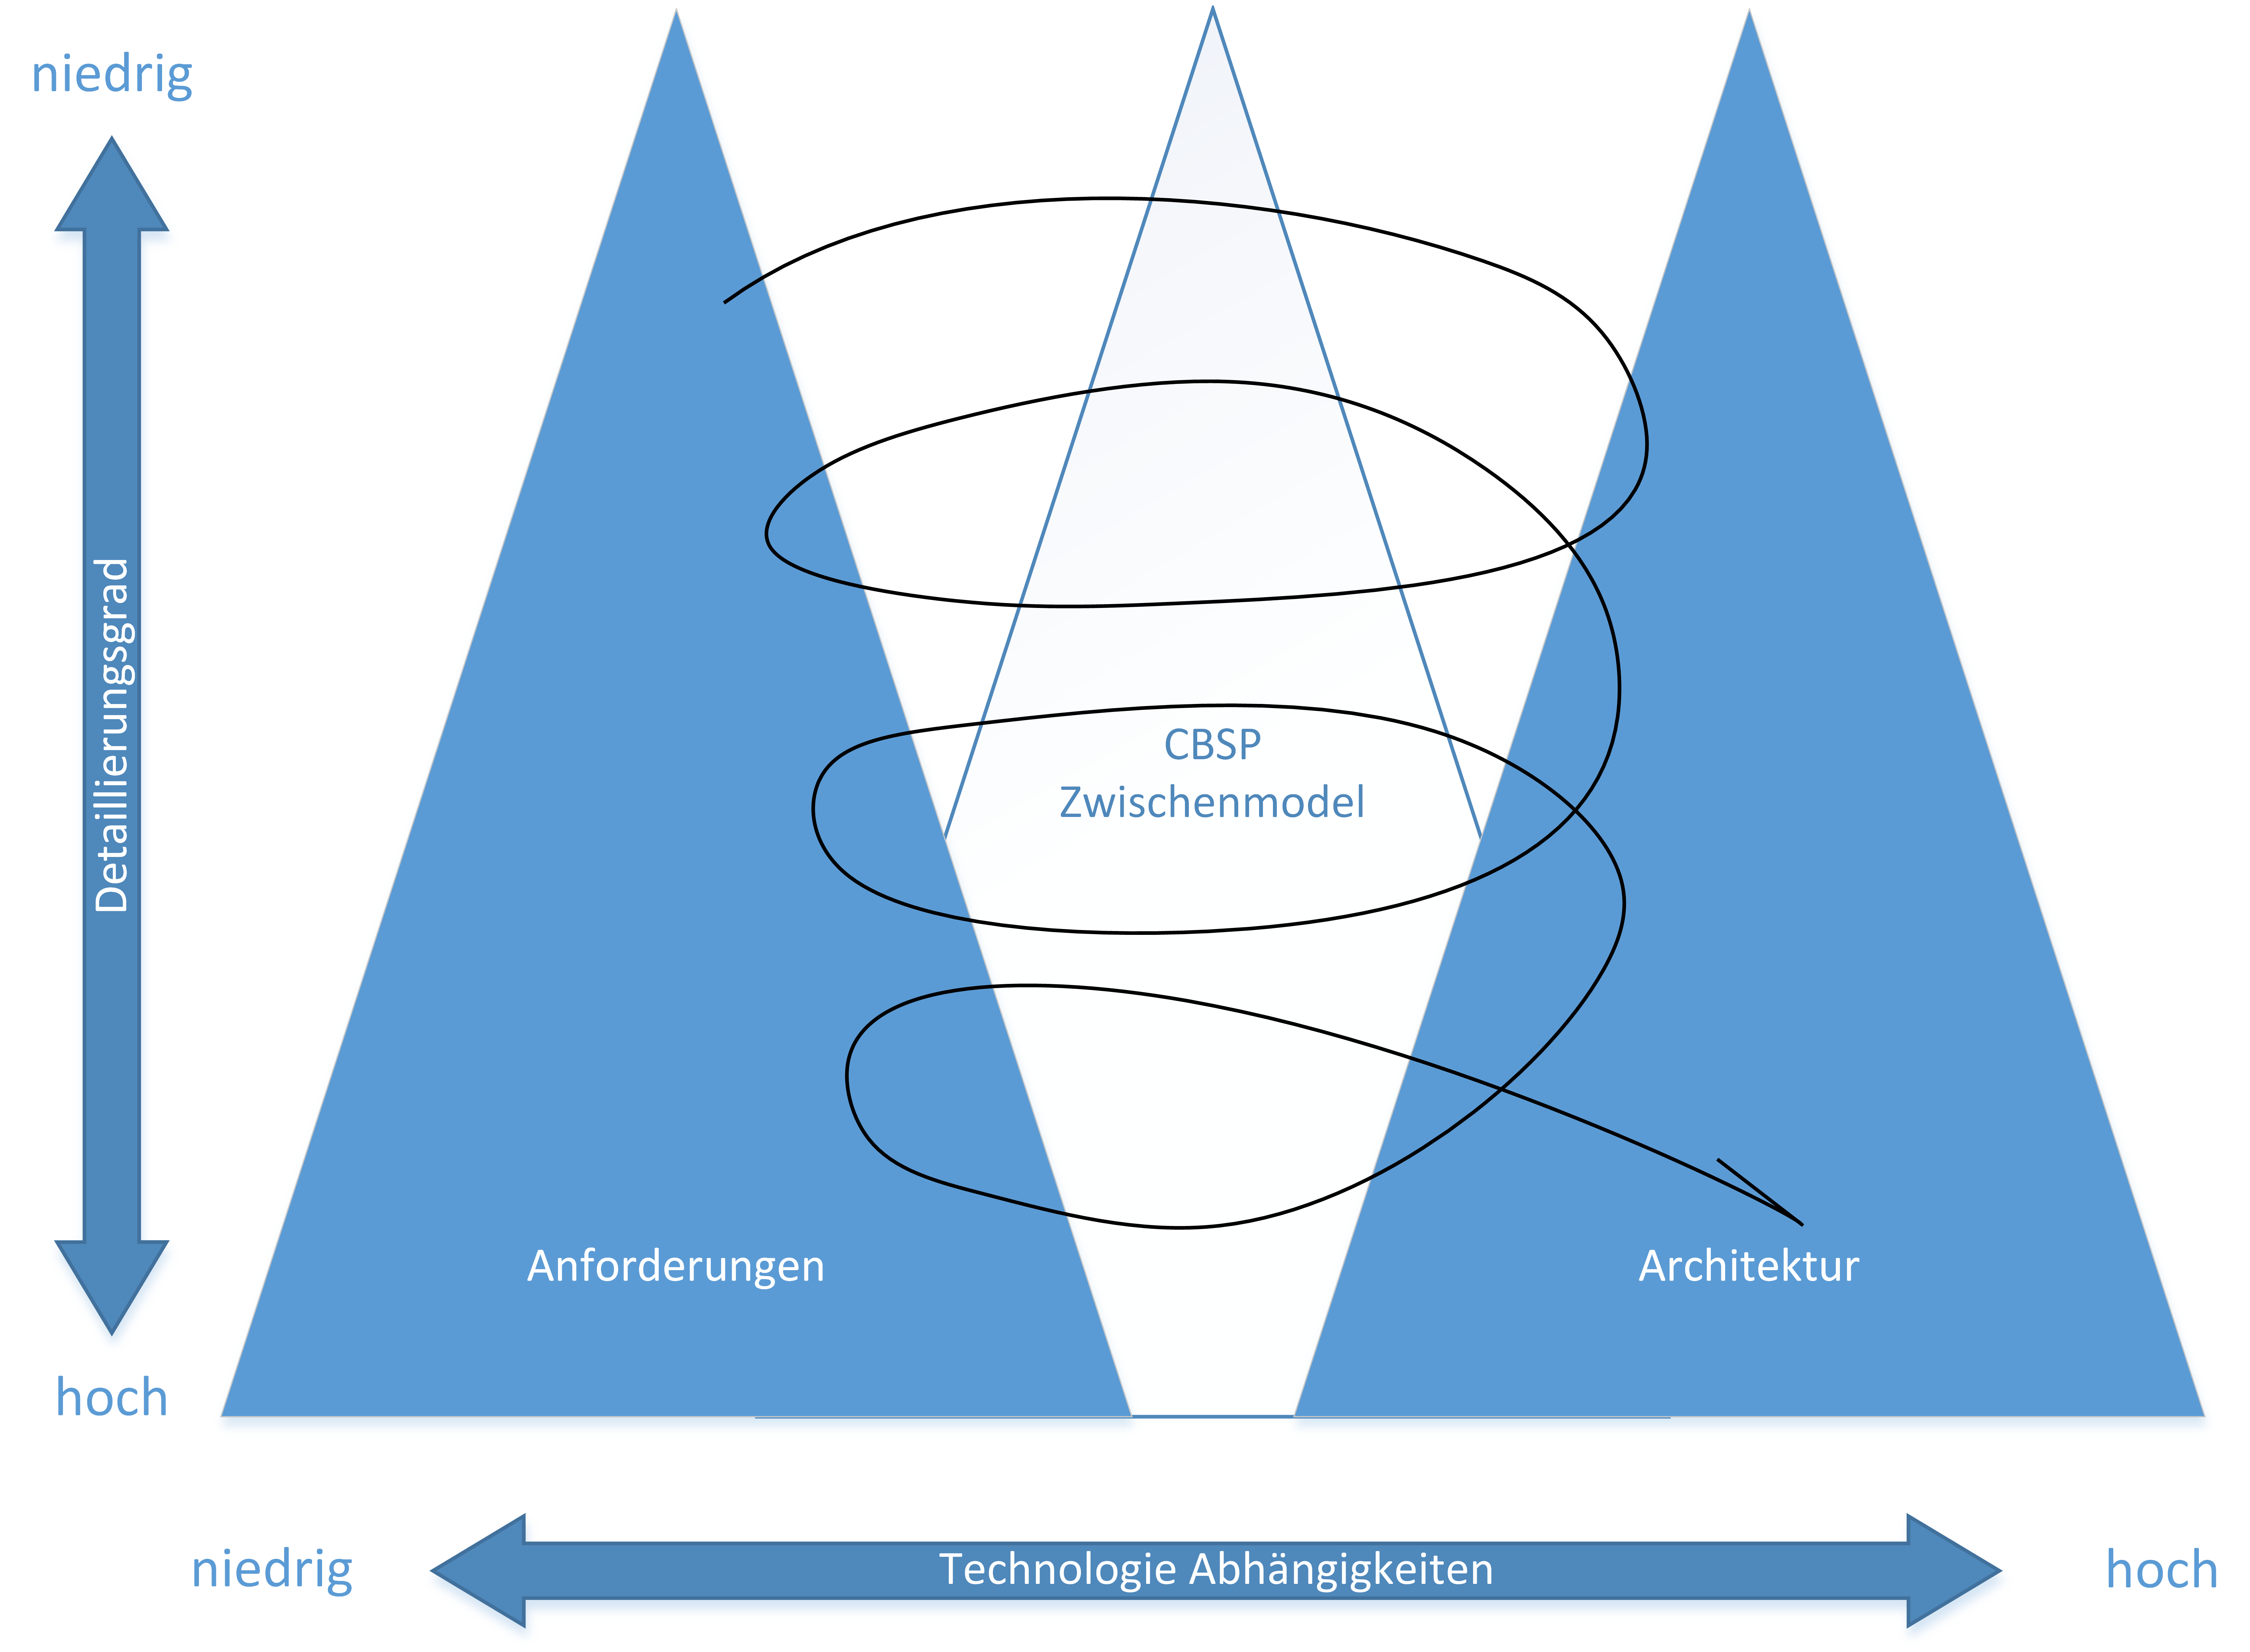
\includegraphics[scale=0.5]{cbsp_model2.png} 
	\caption{CBSP Modell Kontext \cite{Gru01}}
	\label{fig_cbsp_model}
\end{figure}

\emph{CBSP Taxonomie:}
Das Metamodell von CBSP beinhaltet die Basiskonstrukte einer Architektur und ist in sechs Dimensionen aufgeteilt: \\

\begin{itemize}
\item[1.] \textit{C}: sind Elemente, welche individuelle Komponenten der Software-Architektur beschreiben oder involvieren. Diese sind in Datenkomponenten (C\textsubscript{D}) und Verarbeitungskomponenten (C\textsubscript{P}) unterteilt. So k\"onnte beispielsweise die Anforderung: \\
	\textit{R: Benutzern das direkte manipulieren von Kalkulationstabellen erlauben.} \\
	in folgende CBSP Modellelemente verfeinert werden: \\
	\textit{C\textsubscript{P}: UI Komponente f\"ur Kalkulationstabellen Manipulation.} \\
	\textit{C\textsubscript{D}: Daten f\"ur Kalkulationstabellen.}  \cite{Gru01}
\item[2.] \textit{B}: sind Elemente, welche Konnektoren beschreiben. Zum Beispiel: \\
	\textit{R: Manipulierte Daten in Kalkulationstabellen muss im Dateisystem gespeichert werden.} \\
	kann in folgendes CBSP Modellelement verfeinert werden: \\
	\textit{B: Konnektor der die Interaktion zwischen UI und Persistenz-Komponenten erm\"oglicht.} \cite{Gru01}
\item[3.] \textit{S}: sind Elemente, welche systemweite Features beschreiben oder solche, die zu einer gr\"o\ss{}eren Untermenge von Komponenten und Konnektoren passen. Zum Beispiel: \\
	\textit{R: Der Benutzer soll angemessene Filter und Visualisierungen ausw\"ahlen k\"onnen.} \\
	kann in folgendes CBSP Modellelement verfeinert werden: \\
	\textit{S: Das System soll eine strikte Trennung von Datenhaltungs-, -Bearbeitungs- und -Visualisierungs-Komponenten vornehmen.} \cite{Gru01}
\item[4.] \textit{CP}: sind Elemente, welche Eigenschaften, wie Zuverl\"assigkeit, Portabilit\"at, Skalierbarkeit, Anpassbarkeit und Erweiterbarkeit, von Daten- oder Verarbeitungskomponenten beschreiben. Zum Beispiel: \\
	\textit{R: Das Benutzer soll die Daten entfernt mit minimale wahrgenommener Latenz visualisieren k\"onnen.} \\
	kann in folgendes CBSP Modellelement verfeinert werden: \\
	\textit{CP: Die Datenvisualisierungs-Komponente soll effizient sein und inkrementelle Updates unterst\"utzen.} \cite{Gru01}
\item[5.] \textit{BP}: sind Elemente, welche Eigenschaften von Konnektoren beschreiben. Zum Beispiel: \\
	\textit{R: Updates f\"ur Systemfunktionen sollen mit minimaler Ausfallzeit m\"oglich sein.} \\
	kann in folgendes CBSP Modellelement verfeinert werden: \\
	\textit{BP: Robuste Konnektoren sollen zur Verf\"ugung gestellt werden, um das Hinzuf\"ugen und Entfernen von Laufzeitkomponenten zu erleichtern.} \cite{Gru01}
\item[6.] \textit{SP}: sind Elemente, welche systemweite Eigenschaften bzw. Eigenschaften von Subsystemen beschreiben. Zum Beispiel: \\
	\textit{R: Die Daten der Kalkulationstabellen m\"ussen verschl\"usselt werden bevor sie \"uber das Netzwerk versandt werden.} \\
	kann in folgendes CBSP Modellelement verfeinert werden: \\
	\textit{SP: Das System soll sicher sein.} \cite{Gru01} \\
\end{itemize}

Aus diesen Elementen wird das CBSP Zwischenmodell aufgebaut. Das Metamodell zu diesen Elementen ist in Abbildung \ref{fig_cbsp_meta_model} dargestellt. Jedes CBSP Artefakt beschreibt eine architekturrelevantes Anliegen und beschreibt eine fr\"uhe Architekturentscheidung des zu erstellenden Systems \cite{Gru01}. \\

Von einer Anforderung zu einem CBSP Element kann eine Verfeinerung, siehe Beispiel (5), oder Generalisierung, siehe Beispiel (6), erfolgen. Diese beiden m\"oglichen Anpassungen basieren auf Notwendigkeiten, welche durch bestimmte Eigenschaften des zu erstellenden Systems, Charakteristika der Anwendungsdom\"ane oder Hintergrund und Erfahrung des Software-Architekten, erwachsen \cite{Gru01}. Da es f\"ur Verfeinerung und Generalisierung keine allgemeinen formalen Regeln gibt, ist es h\"aufig notwendig hierf\"ur den Kunden bzw. weitere Stakeholder wie den Requirements Engineer zu konsultieren \cite{Gru01}. 

\begin{figure}[h]
	\centering
	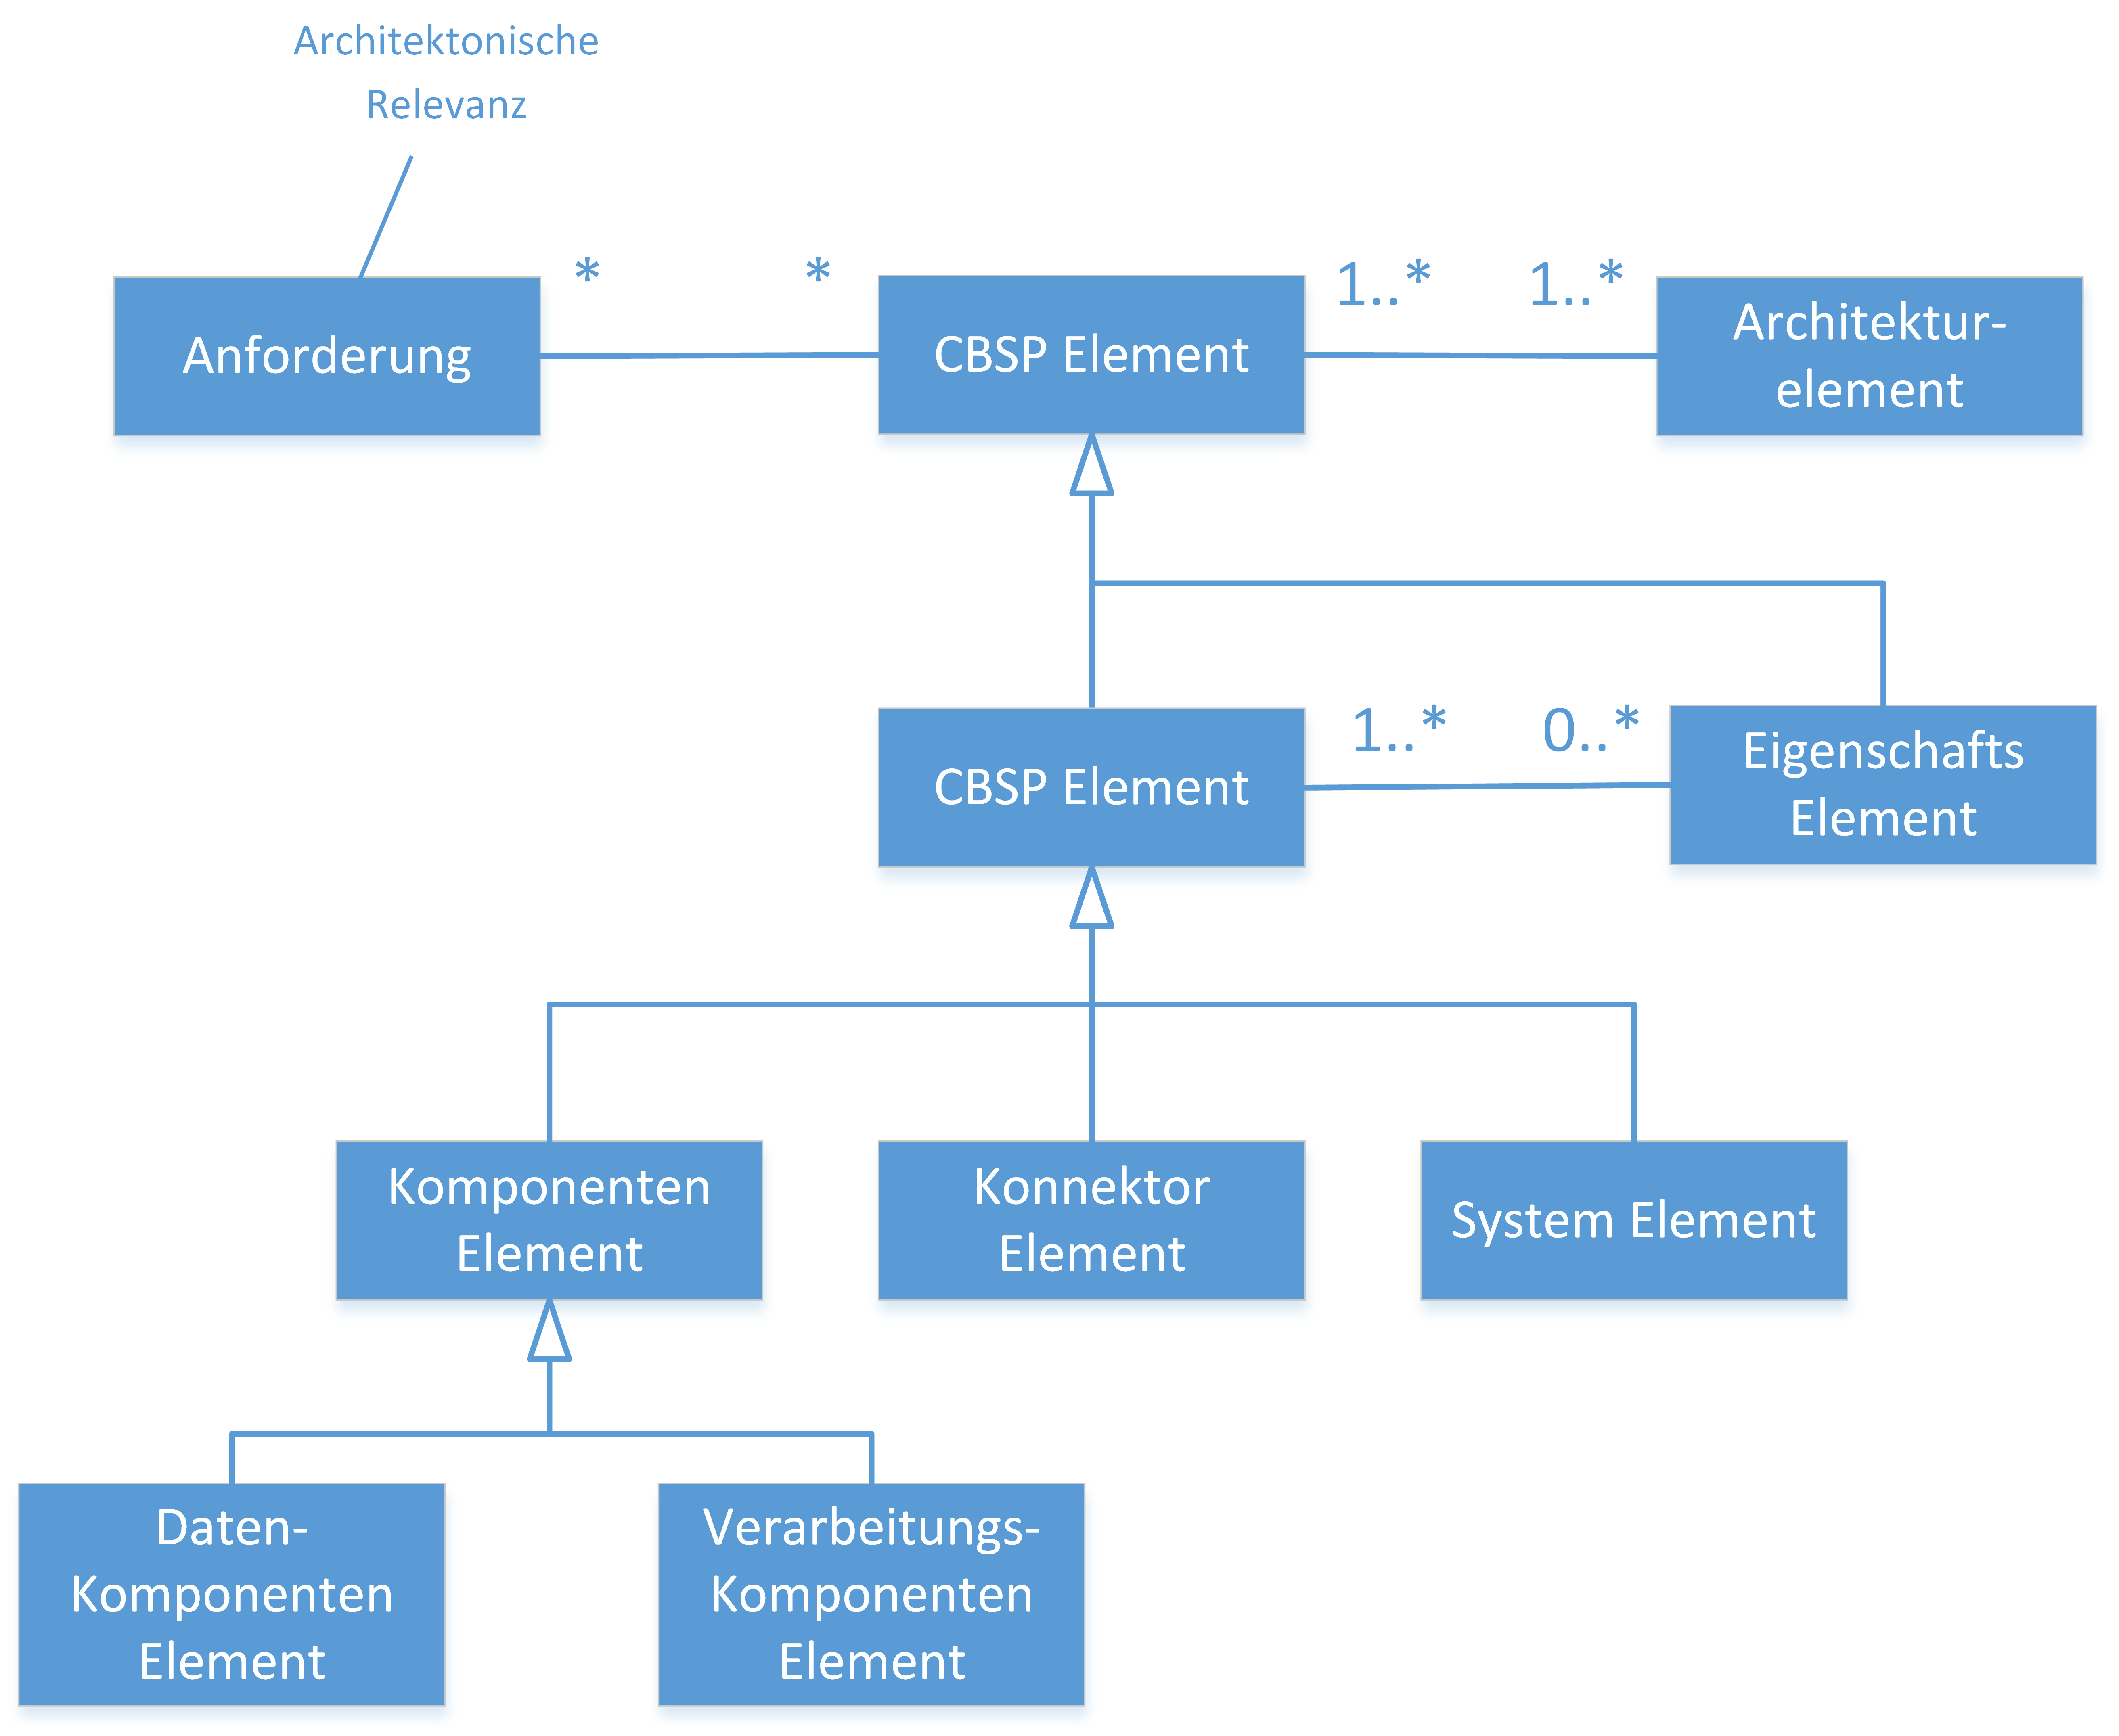
\includegraphics[scale=0.6]{cbsp_meta_model.png} 
	\caption{CBSP Metamodell \cite{Gru01}}
	\label{fig_cbsp_meta_model}
\end{figure}

\paragraph{Randbedingungen}

Damit CBSP erfolgreich angewandt werden kann muss die Bereitschaft zur Mitarbeit aller involvierten Stakeholder gegeben sein. In fast allen Schritten k\"onnen diese bei Unklarheiten oder f\"ur Feedback herangezogen werden. In einigen Schritten ist deren Mitarbeit verpflichtend. \\
Desweiteren m\"ussen die Software-Architekten \"uber ein gewisses Mindestma\ss{} an Erfahrung und Wissen verf\"ugen um die einzelnen Schritte kompetent durchf\"uhren zu k\"onnen. Daf\"ur gibt es allerdings keine Liste mit Mindestvoraussetzungen oder ein Minimum an Jahren an Berufserfahrung. Hier muss klar sein ob der Architekt die n\"otigen Kompetenzen besitzt um wichtige Entscheidungen selbstst\"andig treffen zu k\"onnen. \\

\paragraph{Eingabe}

Als Eingabe ben\"otigt das CBSP eine erste Anforderungsspezifikation. Diese muss noch nicht vollst\"andig sein, denn sie kann in jeder Iteration weiter erg\"anzt werden. Da CBSP nicht auf FRs oder NFRs zugeschnitten ist, werden alle Anforderungen genutzt, denn beide Anforderungstypen haben sowohl explizit als auch implizit Informationen, welche f\"ur die Software-Architektur relevant sind \cite{Gru01}. \\


\paragraph{Vorgehensmodell} 
Jede Iteration von CBSP besteht aus f\"unf Schritten, welche im folgenden vorgestellt werden. \\

\emph{Schritt 1: Auswahl der Anforderungen f\"ur die n\"achste Iteration} - 
Um die Komplexit\"at zu reduzieren werden hier, wie bereits angesprochen, durch ein Team von Architekten nur Anforderungen f\"ur die Iteration ausgew\"ahlt, welche mittels zweier Kriterien durch den Requirements Engineer als wichtig oder durchf\"uhrbar bewertet wurden: (1) die \textit{Bedeutung} zeigt die Relevanz und den Wert f\"ur den Projekterfolg, (2) w\"ahrend die \textit{Durchf\"uhrbarkeit} technische, \"okonomische und politische Bedingungen ber\"ucksichtigt \cite{Gru01}. Diese Anforderungen k\"onnen formell, informell oder semi-formell notiert sein. \\

\emph{Schritt 2: Architektonische Klassifizierung der Anforderungen} - 
In Schritt zwei klassifizieren die Software-Architekten die selektierten Anforderungen mit Hilfe der CBSP Taxonomie. Desweiteren werden alle so klassifizierten Anforderungen in einer Tabelle anhand ihrer Relevanz zu den sechs CBSP Dimensionen bewertet. Die Bewertung erfolgt \"uber eine Ordinalskala (nicht=0; partiell=1; weitgehend=2; voll=3) und beschreibt die Auswirkung, welche die Anforderung auf eine oder mehrere der jeweiligen CBSP Elemente hat \cite{Gru01}. Eine Beispielhafte Bewertung der Anforderungen \textit{R01: Unterschiedliche Ladungstypen unterst\"utzen}, \textit{R02: Verschiedene Fahrzeuge unterst\"utzen} und \textit{R09: Sch\"atzung der Frachtankunft und Fahrzeugverf\"ugbarkeit unterst\"utzen} ist Tabelle \ref{tab:relevance_profiles} zu entnehmen \cite{Gru01}. 

\begin{table}[h] %h, t, b, p : here = genau an dieser Stelle, wenn m\"oglich, top = f\"ur den Seitenanfang, bottom = f\"ur das Seitenende, p = f\"ur eine spezielle Seite mit Tabellen und Abbildungen
\caption{Beispiel Relevanzprofile nach \cite{Gru01}}
\centering
\begin{tabular}{|l|c|c|c|c|c|c|}
\hline 
\textbf{Anforderungen} & \textbf{C} & \textbf{B} & \textbf{S} & \textbf{CP} & \textbf{BP} & \textbf{SP} \\ 
\hline 
R01 & 1,33 & 0,33 & \cellcolor{Gray} 1,67 & 1,00 & 0,33 & 0,33 \\ 
\hline 
R02 & \cellcolor{Gray} 2,00 & 0,00 & 1,00 & 1,33 & 0,00 & 0,00 \\ 
\hline 
R09 & \cellcolor{Gray} 2,67 & 1,33 & 2,00 & 0,33 & 0,00 & 0,00 \\ 
\hline 
\end{tabular} 
\label{tab:relevance_profiles}
\end{table}

\begin{table*}[t] %h, t, b, p : here = genau an dieser Stelle, wenn m\"oglich, top = f\"ur den Seitenanfang, bottom = f\"ur das Seitenende, p = f\"ur eine spezielle Seite mit Tabellen und Abbildungen
\caption{CBSP zu Architekturstil Mapping nach \cite{Gru01}}
\centering
\newcolumntype{M}[1]{>{\centering\arraybackslash}p{#1cm}}
\begin{tabular}{|p{3cm}|p{4,2cm}|M{2}|M{1}|M{2}|M{1,5}|M{1,3}|}%{|l|c|c|c|c|c|c|} 15
\hline 
\textbf{CBSP Dimensionen} & \textbf{Eigenschaften} & \textbf{Client-Server} & \textbf{C2} & \textbf{Event-basiert} & \textbf{Schichten-Architektur} & \textbf{Pipes und Filter} \\ 
\hline 
Datenkomponente & aggregiert & ++ & ++ & ++ & + & - \\ 
 & persistent & ++ & o & o & o & o \\ 
 & gestreamt & - & - & - & - & + \\ 
 & gecached & ++ & + & - & - & - \\ 
\hline 
Verarbeitungskomponente & Dienste anbieten / Nur konsumieren & ++ & o & o & o & o \\ 
 & hat N Schnittstellen & ++ & + & ++ & - & - \\ 
 & stateful & + & ++ & ++ & + & - \\ 
 & lose gekoppelt & + & + & ++ & - & ++ \\ 
 & kann migriert werden & + & ++ & ++ & - & - \\ 
\hline 
Konnektor & synchron & ++ & - & + & ++ & - \\ 
 & asynchron & - & ++ & ++ & - & ++ \\ 
 & lokal & - & ++ & o & ++ & + \\ 
 & verteilt & ++ & ++ & ++ & - & + \\ 
 & sicher & + & o & o & + & o \\ 
\hline 
(Sub-)System & effizient & o & + & + & o & - \\ 
 & skalierbar & + & o & - & - & + \\ 
 & weiterentwickelbar & ++ & ++ & ++ & - & ++ \\ 
 & portierbar & o & + & o & ++ & o \\ 
 & zuverl\"assig & o & o & - & o & o \\ 
 & dynamisch & + & ++ & ++ & - & ++ \\
\hline 
\end{tabular} 
\label{tab:cbsp_to_style_mapping}
\end{table*}

\emph{Schritt 3: Identifizierung und Aufl\"osung von falschen Zuordnungen bei der Klassifizierung} - 
Da mehrere Software-Architekten diese Klassifizierung unabh\"angig voneinander vornehmen, m\"ussen im dritten Schritt m\"ogliche Abweichungen aufgedeckt, diskutiert und behoben werden. Dies ist wichtig um Missverst\"andnisse, mehrdeutige Anforderungen, implizites Wissen, und widerspr\"uchliche Auffassungen zu identifizieren und Risiken bei der Verfeinerung der Anforderungen zu reduzieren \cite{Gru01}. Bei der Diskussion k\"onnen auch der Kunde und Requirements Engineer involviert sein. Der erarbeitete Konsens sorgt f\"ur ein einheitliches Verst\"andnis der Anforderungen und die Relevanz dieser f\"ur die Software-Architektur. Wenn keine Unstimmigkeiten mehr vorliegen werden die Anforderungen weiter ausged\"unnt indem alle Anforderungen, welche eine geringere Relevanz haben als ein vorher definierter Wert der Ordinalskala, wie beispielsweise "weitgehend", vorerst verworfen werden. Dabei wird auf Abh\"angigkeiten zwischen den Anforderungen geachtet um kritische nicht zu verwerfen. Alle akzeptierten Anforderungen werden inklusive gesammelter Probleme und Unklarheiten in den n\"achsten Schritt \"ubernommen. \\

\emph{Schritt 4: Architektonische Verfeinerung der Anforderungen} - 
Im vorletzten Schritt werden die CBSP Elemente umformuliert oder aufgeteilt, welche \"uberlappende CBSP Dimensionen und architektonische Anliegen aufweisen. Wenn ein CBSP Element beispielsweise weitgehend Komponenten-relevant, voll Konnektor-relevant und weitgehend Konnektor-Eigenschafts-relevant ist, erh\"oht es das Verst\"andnis und die Pr\"azision wenn es in mehrere Architekturentscheidungen, verk\"orpert als CBSP Element, aufgesplittet wird. Ein einzelnes CBSP Artefakt kann w\"ahrend diesem Prozess mehrfach als Nebenprodukt bei verschiedenen Anforderungen auftauchen, w\"ahrend diese Redundanzen identifiziert und eliminiert werden \cite{Gru01}. \\

In diesem Schritt gibt es zwei Varianten welche entweder einzeln oder sogar kombiniert ausgef\"uhrt werden k\"onnen. Variante eins betrachtet zun\"achst nur die gro\ss{}en strukturellen Aspekte des Systems (C, B und S Elemente). Dies hat den Vorteil, dass der Architekt leichter einen Überblick behalten kann, da die beiden Aspekte (Struktur und Funktionalit\"at vs. nicht-funktionale Eigenschaften) separat betrachtet werden. Die Eigenschaften der drei Elemente werden in einem gesonderten (Sub-)Prozess identifiziert. Die zweite Variante identifiziert in einem Schritt sowohl die strukturellen Elemente als auch ihre nicht-funktionalen Eigenschaften. Der Vorteil hierbei ist, dass der Software-Architekt sich auf ein kompletten System Aspekt (oder eine kleine Menge von Aspekten) konzentrieren kann. \\

\emph{Schritt 5: Abgleich der Entscheidungen zwischen Architekturelementen und -stilen mit CBSP} - 
Wenn alle ausgew\"ahlten Anforderungen im CBSP Model modelliert wurden, sodass keine Konflikte zwischen Software-Architekt und Requirements Engineer bestehen und alle CBSP Modellelementen weitgehend relevant zu einer der sechs CBSP Dimensionen sind, kann in Schritt f\"unf ein erster Architektur-Prototyp abgeleitet werden. \\
Die Bestimmung eines passenden Architekturstiles mit den zu den CBSP Modellelementen passenden Architekturmustern ist nicht immer einfach. Zum einen existiert kein formaler Ansatz f\"ur diesen Prozess, zum anderen k\"onnen mehrere Architekturstile zum generierten CBSP Modell passen. F\"ur diese Aufgabe gibt es verschiedene Verfahren. Hier wird die Selektion eines passenden Architekturstiles mit Hilfe einer Matrix aufgestellt, siehe Tabelle \ref{tab:cbsp_to_style_mapping}. Diese Metrix stellt die CBSP Dimensionen mit geeigneten Eigenschaften potentiellen Architekturmustern gegen\"uber. Allerdings ist diese Tabelle nicht vollst\"andig, denn weitere Eigenschaften f\"ur die CBSP Elemente sind denkbar und es werden auch nicht alle existierenden Architekturstile angeboten. Zum einen ist sie daf\"ur nicht gedacht, sie soll lediglich eine Hilfestellung bei der Wahl eines passenden Architekturstils bieten sobald mehr als einer passend erscheint. Daf\"ur muss sie nur so umfassend wie eben n\"otig sein. Zum anderen w\"urde eine vollst\"andige Tabelle \textit{jedes} Softwaresystem darstellen und nicht auf eine konkrete Dom\"ane zurecht geschnitten sein. Au\ss{}erdem w\"are eine solche unm\"oglich zu erstellen \cite{Gru01}. Die endg\"ultige Wahl liegt allerdings beim Software-Architekten. \\

Anschlie\ss{}end muss der Software-Architekt die CBSP Modellelemente in entsprechende Architekturelemente wie Komponenten, Konnektoren, Konfigurationen, Pakete und Daten mit den gew\"unschten Eigenschaften umwandeln \cite{Gru01}. \\

\paragraph{Ausgabe}

Nach der Ausf\"uhrung der f\"unf Schritte und mehrfachen Iterationen sollte eine Software-Architektur gegeben sein, welche die selektierten Anforderungen zu einem m\"oglichst hohen Grad erf\"ullt.

%\textbf{Paper Cites:} \\
%(\cite{Gru01}) Reconciling software requirements and architectures with intermediate models \\


%Viel ^^ (Weaving the Software Development Process Between Requirements and Architectures)

%RE und SA sind sehr voneinander abh\"angig (Descending the twin Peaks)


%\begin{itemize}
%\item[1.] Text
%\item[2.] Text
%\item[3.] Text \\
%\end{itemize}
\subsection{sCenario and gOal based SysteM develOpment methoD (COSMOD) (FDD)}\label{scgo}
COSMOD-Requirements Engineering (COSMOD-RE) beschreibt ein iteratives Vorgehen zum gleichzeitigen Design von Anforderungen und Software-Architektur. Kerngedanke bei COSMOD-RE ist eine Aufteilung in vier Hierarchiestufen, wo sowohl Architektur als auch Anforderungen definiert werden. In diesen vier Hierarchiestufen wird einerseits aus der Anforderungssicht und andererseits aus der Architektursicht betrachtet, welche Anforderungen und Komponenten dem System zuzuordnen sind.
\subsubsection{Ziele der Methode}
Kernziel von COSMOD-RE ist es die Entwicklung von Anforderungs- und Architekturartefakten für softwareintensive eingebettete Systeme zu unterstützen. Ein Ziel- und Szenario-basierter Ansatz wie COSMOD-RE, der das Co-Design von Architekturartefakten und Anforderungen ermöglicht muss jedoch einige Anforderungen erfüllen um einen Nutzen zu haben. Die Anforderungen an eine solchen Methodik sind \cite{pohl}\\
 
\begin{itemize}
\item Parallele Entwicklung von Anforderungen und Architekturartefakten \\
Da Anforderungen und die Software Architektur die Kerntreiber hinter innovativen Projekten sind ist es wichtig beide gleichermaßen zu nutzen, sodass keines von beiden in den Vordergrund tritt \cite{pohl}.
\item Unterstützung der Anordnung von Anforderungen und Architekturartefakten \\
Werden Anforderungen und Architekturartefakte parallel entwickelt kann es passieren, dass Inkonsistenzen auftreten. Um diese zu vermeiden ist es notwendig, dass COSMOD-RE diese erkennt und behebt \cite{pohl}.
\item Definition detaillierter Anforderungen auf der Basis von Architekturartefakten \\
Ohne technisches Wissen fällt es Stakeholdern schwer notwendige Details für die Erhebung architekturrelevanter Anforderungen zu liefern. Daher sollte es COSMOD-RE ermöglichen die detaillierten Anforderungen erst nach der initialen Definition von Architekturartefakten zu liefern \cite{pohl}. 
\item Nutzung einer Abstraktionshierarchie \\
Da bei einem Co-Design Vorgehen eine große Komplexität bestehen kann ist es notwendig eine Abstraktionshierarchie einzuführen um diese entsprechend zu behandeln \cite{pohl}.\\
\end{itemize}

\subsubsection{Funktionsweise der Methode}
Das wichtigste Element von COSMOD-RE ist die Abstraktionshierarchie. Über diese werden alle Aktivitäten die im Rahmen der Methodik stattfinden eingeordnet und miteinander in einen Kontext gesetzt. So wird auf jeder Ebene der Abstraktionshierarchie eine Architektursicht und eine Anforderungssicht erzeugt. Hierbei ist jedoch zu beachten, dass bei COSMOD-RE nicht unbedingt ein Top-Down-Ansatz zu wählen ist, da Anforderungsartefakte und Architekturartefakte auf allen Ebenen gleichzeitig bearbeitet werden können.\\

\paragraph{Randbedingungen}
Bei der Anwendung von COSMOD-RE ist zu beachten, dass einige Bedingungen erfüllt sein müssen um die Methodik richtig anzuwenden:\\

\begin{itemize}
\item Definition einer Abstraktionshierarchie \\
Es gibt keine Richtlinien bezüglich der Definition der Abstraktionshierarchie. Dies bedeutet, dass die verwendeten Hierarchiestufen im jedem Projekt neu festgelegt werden müssen. Ferner ist hierbei von Relevanz, zu definieren, wo die Trennlinien zwischen verschiedenen Abstraktionsstufen sind \cite{sikora}.
\item Verknüpfung von Anforderungs- und Architekturmodellen \\
Da im Rahmen von COSMOD-RE Anforderungsartefakte und Architekturartefakte parallel entwickelt werden ist es notwendig diese miteinander zu verknüpfen um sie in den Kontext des Ziels der Software zu bringen. Für diese Verknüpfung ist die Anwendung von Methodenfragmenten notwendig \cite{sikora}.
\item Definition von Konsistenzbedingungen \\
Für die Definition von Konsistenzbedingungen gibt es keinen allgemeingültigen Ansatz. Daher ist es notwendig in jedem Projekt neu zu definieren, ob Konsistenz gegeben ist oder nicht \cite{sikora}.\\
\end{itemize}

Sind diese Randbedingungen geklärt ist es möglich COSMOD-RE anzuwenden.\\

\paragraph{Eingabe}

\paragraph{Vorgehensmodell}
\paragraph{Ausgabe}

\subsubsection{Beschreibung}
In der Anforderungserhebung soll es m\"oglich sein Anforderungen in einer Form zu erheben, die es Software Architekten einfacher macht, den Architekturentwurf zu konzipieren. Um dies zu realisieren bietet sich eine Kombination aus Ziel-basierten Ans\"atzen und Szenario-basierten Ans\"atzen an. Die Kombination ist deswegen von Relevanz, weil ein Ansatz allein nicht ausreichen kann um die Anforderungen in angemessener Weise zu erheben.\\

\subsubsection{Ziel-basierte Ans\"atze}
Ziel-basierte Ans\"atze zielen vorrangig darauf ab, ein umfassendes Verst\"andnis der W\"unsche und Ziele der Stakeholder sowie auf die zu erzielenden Auswirkungen auf die Systemumgebung ab (Silkora Referenz S.18). Dies bedeutet, dass es bei Ziel-basierten Ans\"atzen vor allem darauf ankommt, zu verstehen, welche Vision der Stakeholder von dem Zuk\"unftigen System hat. Bei der Erfassung dieser Vision ist ein nat\"urlichsprachlicher Ansatz fehlerbehaftet, da hier sehr aufw\"andige manuelle Konsistenzpr\"ufungen notwendig w\"aren. Deswegen bieten sich hier vor allem Modell-basierte Ans\"atze an.\\

Ein gutes Beispiel f\"ur ein Modell-basierten Ansatz ist der KAOS-Ansatz. Dieser Ansatz bietet den Vorteil, dass er mit wenigen pr\"azise formulierten Modellierungsobjekten auskommt. Dies ist deswegen ein Vorteil, weil so kein besonders tief reichendes Fachwissen notwendig ist um das Modell zu interpretieren. Ferner ist der Ansatz f\"ur die Konzeption softwareintensiver eingebetteter Systeme geeignet, was eine verzahnte Entwicklung von Anforderungen und Architektur \"uber mehrere Abstraktionsstufen hinweg erm\"oglicht (Silkora Referenz S.31).\\

\paragraph{KAOS}
Lamsweerde (Lamsweerde Referenz) beschreibt eine modellbasierten Ansatz zur Darstellung von Zielen und den Referenzen innerhalb von Zielen. Hierf\"ur muss zun\"achst eine genauere Betrachtung der Zieldefinition vorgenommen werden. So sind in dem Kontext der KAOS-Methode Ziele in Bahavioral-Goals und Soft-Goals zu unterteilen. \\

Behavioral-Goals beschreiben eine deklarative Sicht auf Ziele, die beschreibt, wie ein System sich zu verhalten hat. Dies bedeutet, dass in diesem Fall besonders das Verhalten von Systemen im Fokus steht. G\"ultig ist eine endliche Menge von Verhaltensweisen des Systems. \\

Grunds\"atzlich lassen sich Bahavioral-Goals in zwei Kategorien aufteilen, die Achive-Goals und die Maintain/Avoid-Goals. Die Achive-Goals beschreiben Systemverhalten, bei dem es darauf ankommt, dass ein System zu einem definierten Zeitpunkt einen definierten Zustand erreicht. Maintain/Avoid-Goals beschreiben Systemverhalten, bei dem es darauf ankommt, dass ein System \"uber einen definierten Zeitraum hinweg einen definierten Zustand aufrechterh\"alt, oder einen definierten Zustand vermeidet.\\

Soft-goals beschreiben Pr\"aferenzen innerhalb von g\"ultigen Systemverhaltensweisen. Diese lassen sich zun\"achst in funktionale Ziele und nicht funktionale Ziele aufteilen. Die funktionalen Ziele k\"onnen die folgenden Kategorien haben:
\begin{itemize}
\item Satisfaction: Funtionale Ziele, die sich damit besch\"aftigen User-Anfragen zu beantworten.
\item Information: Funtionale Ziele, die damit besch\"aftigt sind User \"uber wichtige Systemzust\"ande zu informieren.
\item Stim-response: Funktionale Ziele, die sich damit besch\"aftigen auf Events eine angemessene Reaktion zu erzeugen.
\end{itemize}
Mit dem gegebenen Ziel die Zusammenarbeit zwischen Requirements Engineer und Software Architekt zu optimieren sind vor allem die funktionalen Ziele der Soft-Goals und die Behavioral-Goals von Relevanz.\\

der KAOS Ansatz, der die zuvor beschriebenen Zielarten als Grundlage nutzt, verwendet zur Modellierung Und-/Oder-Graphen, die in diesem Kontext Zieldiagramm genannt werden. Jedes im Graphen modellierte Ziel wird zun\"achst durch eine Reihe von Eigenschaften in einer Zielschablone charakterisiert. Die Eigenschaften k\"onnen unter anderem Name, Definition, Quelle, Zielkategorie und Priorit\"at sein.\\

--TODO-- Erzeugung Abbildung Und-Oder-Graph + Beschreibung der Elemente\\

Das Problem von Ziel-basierten Ans\"atzen wie dem KAOS Ansatz ist, dass eine Software Architektur allein basierend auf den Zielen wichtige Aspekte vernachl\"assigt. So zum Beispiel welche Rolle diese Ziele erreichen soll und gegebenenfalls wie die dieses Ziel umzusetzen ist. Daher ist es notwendig Szenario-basierte Ans\"atze zu betrachten.\\

\subsubsection{Szenario-basierte Ans\"atze}
Szenario-basierte Ans\"atze zielen vorrangig darauf ab, die wesentlichen geforderten Interaktionen des Systems mit dessen Umgebung zu definieren und mit den Stakeholdern abzustimmen (Silkora Referenz S.18).\\

Um die optimale Zusammenarbeit zu st\"utzen ist es notwendig, die Szenarien in einer Kombination aus Anwendungsfalldiagrammen und Message Sequence Charts graphisch zu modellieren. Dadurch, kann der Zusammenhang zwischen Szenarien aufgezeigt werden und wichtige Aspekte, die von Bedeutung f\"ur den Design der Softwarearchitektur sind, ber\"ucksichtigt werden. Es ist mit diesem Vorgehen m\"oglich Szenarien zu komplexeren Szenarien zusammenzusetzen und des weiteren Iterationen und alternative Szenarienverl\"aufe abzubilden (Silkora Referenz S.33). Bei der Betrachtung von Szenarien ist es jedoch auch hier notwendig, diese zun\"achst in Schablonen zu dokumentieren, um eine pr\"azise Beschreibung zu haben. In einer Schablone soll unter anderem festgehalten werden, welche prim\"aren und sekund\"aren Akteure gegeben sind. Ferner sollen eine Kurzbeschreibung und mit dem Szenario verkn\"upfte Ziele gegeben sein, um klar hervorzuheben, in welchem Kontext das Szenario zu sehen ist.\\

\paragraph{Anwendungsfalldiagramm}
Das Anwendungsfalldiagramm zeigt eine \"Ubersicht \"uber die Anwendungsf\"alle eines Systems oder einer Systemkomponente. Es stellt zudem die Akteure des Systems (der Komponente) und deren Beteiligung an den Anwendungsf\"allen grafisch dar (Silkora Zitat S.34). \\

Anwendungsf\"alle k\"onnen als Oberbegriff f\"ur Szenarien betrachtet werden, da ein Szenario sich aus einem Anwendungsfall generieren l\"asst. Dies bedeutet ein Anwendungsfall kann Grundlage für eine Vielzahl von Szenarien sein. \\

--TODO-- Anwendungsfalldiagramm beispielabbildung mit Notationselementen\\

Zu den Notationselementen eines Anwendungsfalldiagramms z\"ahlen:
\begin{itemize}
\item Akteur: Als Akteur l\"asst sich eine Person oder Entit\"at bezeichnen, die mit dem zu konzipierenden System in Beziehung steht. Diese k\"onnen zum Beispiel Nutzer sein, die \"uber eine Eingabemaske Daten eintragen sollen.
\item Systemgrenze: Systemgrenzen umschlie\ss{}en das geplante System. Akteure, die mit dem System interagieren befinden sich au\ss{}erhalb der Systemgrenze, w\"ahrend die dem System zugeordneten Anwendungsf\"alle sich innerhalb der Systemgrenze befinden.
\item Anwendungsfall: Ein Anwendungsfall beschreibt eine Funktionalit\"at des geplanten Systems. In Kombination mit dem Akteur, der in Relation zu einem Anwendungsfall steht, wird dargestellt, was das System machen soll.
\item Erweiterung eines Anwendungsfalls: Ein Anwendungsfall kann mittels Include- oder Extend-Beziehung erweitert werden. Dies soll es erm\"oglichen komplexere Anwendungsf\"alle abzubilden und gleichzeitig die Anzahl der Redundanzen m\"oglichst gering halten. Eine Include-Beziehung bedeutet hierbei, dass ein Anwendungsfall einen weiteren Anwendungsfall beinhaltet. Die Extend-Beziehung bedeutet, dass es zu einem Anwendungsfall eine Erweiterung unter einer Bedingung gibt. Die Bedingung gibt an welche Konditionen erfüllt sein müssen dass die Erweiterung greift.
\end{itemize}
Anwendungsfalldiagramme stellen Akteure und Anwendungsfälle dar. Dadurch wird veranschaulicht welche Akteure mit welchen Anwendungsfällen in Beziehung stehen und ob es wichtige Beziehungen zwischen verschiedenen Anwendungsfällen gibt. Grundsätzlich ist es möglich Anwendungsfalldiagramme auf verschiedenen Abstraktionsstufen abzubilden um so sowohl für das Gesamtsystem, als auch für die Teilsysteme die Beziehungen zu betrachten. Um jedoch Szenarien präzise zu spezifizieren reichen Anwendungsfalldiagramme nicht aus.\\

\paragraph{Message-Sequence-Charts}
Mithilfe von Message-Sequence-Charts ist es möglich eine präzise Spezifikation der verschiedenen Szenarien eines Anwendungsfalls zu generieren (Silkora Zitat S.37). Bei der Betrachtung der Zusammenarbeit zwischen Software-Architekt und Requirements-Engineer ist zunächst nur eine Teilmenge der Notationselemente der Message-Sequence-Charts relevant. Wichtigster Aspekt der Message-Sequence-Charts ist, dass diese vor allem die Akteure und ihre Interaktionen mit dem System hervorheben.\\

Grundsätzlich werde in einem Message-Sequence-Chart Nachrichten und Instanzen abgebildet. Eine Instanz kann hierbei z.B. ein System oder ein Akteur sein. Als Nachricht wird im Kontext der Message-Sequence-Charts der Austausch einer Information bezeichnet. Dies können z.B. Signale oder Daten sein, die zwischen den Instanzen versendet werden (Silkora Referenz S.38). \\

--TODO-- Abbildung zu MSC und Beschreibung\\

Neben den einfachen Message-Sequence-Charts gibt es High-Level-Message-Sequence-Charts (HLMSC), die es ermöglichen eine Komposition mehrerer Message-Sequence-Charts zu bilden und so komplexere Zusammenhänge darzustellen. Grundsätzlich besteht ein HLMSC aus einem Start- und Endknoten, einem oder mehreren Verweisknoten und einer Menge von Kanten. Die Start- und Endknoten dienen hierbei der Begrenzung des Anwendungsfalls.  Die Verweisknoten sind als Verweise zu einfachen Message-Sequence-Charts oder weiteren HLMSC zu sehen. Ungerichtete Kanten dienen der Darstellung der Komposition und mithilfe von gerichteten Kanten lässt sich Iteration darstellen.\\

--TODO-- Abbildung zu HLMSC \\

Wenn Anwendungsfälle in Kompositionen zusammengefasst werden lässt sich argumentieren, dass man bei hinreichenden Kompositionen in den Bereich der Ziele gelangt. Somit wird deutlich, dass der Szenario-basierte Ansatze implizit schon eine Betrachtung der Ziele fordert.\\

\subsubsection{Kombination der Ans\"atze}
Wenn die wesentlichen Ziele der Stakeholder bekannt sind, besteht die M\"oglichkeit, diejenige Architekturalternative auszuw\"ahlen, mit der die Ziele am besten erf\"ullt werden k\"onnen (Silkora Referenz S.18).\\

Sowohl Ziel-basierte Ansätze als auch Szenario-basierte Ansätze sind alleinstehend nicht ausreichend, um eine Grundlage für einen guten Architekturansatz auf der Basis von Anforderungen zu generieren. Hierfür ist es notwendig, die Ansätze zu kombinieren. \\

Ein Beispiel für eine solche Kombination ist der COSMOD-RE (sCenario and gOal based SysteM develOpment methoD) Ansatz. \\

\paragraph{COSMOD-RE}

\begin{itemize}
\item[1] System: Die Systemebene beschreibt die oberste Ebene, bei der in der Anforderungssicht das System als ganzes betrachtet wird. Im Fokus stehen dabei die Interaktionen mit dem System. Weiter werden funktionale Anforderungen und Qualitätsanforderungen erstellt, die sich auf das Gesamtsystem beziehen. Die Architektursicht konzentriert sich hier auf die Definition von externen Systemschnittstellen. Hier definierte Artefakte sollen primär die Kommunikation mit Stakeholdern unterstützen.
\item[2] Komponenten: Die Komponentenebene bezeichnet die Aufteilung des Systems in einzelne Komponenten aus denen sich dieses zusammensetzen soll. Für jede Komponente werden funktionale Anforderungen und Qualitätsanforderungen formuliert. Da in dieser Ebene die Basis für die Systemarchtitektur gelegt wird, hat die Kommunikation zwischen dem Software-Architekten und dem Requirements Engineer von besonderer Bedeutung. 
\item[3] Hard-/Software Komponenten: Auf dieser Ebene werden die zuvor erstellten Komponenten in Hard- und Software Komponenten aufgeteilt und weiter verfeinert. Anforderungen auf dieser Ebene sind somit speziell auf die Komponentenart bezogen. 
\item[4] Deployment: Auf dieser Ebene werden Softwarekomponenten programmierbaren Hardwarekomponeten zugeordnet. Anforderungen auf dieser Ebene beziehen sich auf das Deployment der Softwarekomponenten und ihrem Einfluss auf vorher definierte Anforderungen. 
\end{itemize}
Da die Zusammenarbeit zwischen Software-Architekt und Requirements Engineer vor allem in den obersten beiden Ebenen von Relevanz ist, sind die unteren beiden Ebenen in diesem Kontext zu vernachlässigen.\\

Im Rahmen der Erstellung der Software-Architektur und der Anforderungen gibt es drei Co-Design Prozesse die sich wiederum in fünf Sub-Prozesse unterteilen lassen. Bei Ausführung der Prozesse werden als Artefakte sowohl die System-Architektur als auch Ziele, Szenarien und Anforderungen erzeugt. \\

--TODO-- Abbildung Zu den Sub-prozessen des Designs\\

\subsubsection{Bewertung}
In der Betrachtung Ziel-basierter Ansätze wird deutlich, dass diese allein nicht ausreichen um weitreichende Architekturentscheidungen zu treffen. Hauptproblem ist hier, dass mithilfe der Ziele lediglich angegeben wird, was am Ende aus der Sicht der Stakeholder erreicht werden soll und nicht konkret welche Rolle in dem System welche Aufgaben hat und wie das Ziel zu erreichen ist.\\

Szenario-basierte Ansätze deuten an, dass diese alleinstehend ebenfalls nicht ausreichen um eine Software-Architektur zu entwerfen, da hier vor allem das Problem besteht, dass alleinstehende Szenarien ohne Zusammenhang am Ende der Entwicklung keine konsistentes System ergeben können. Durch Ziele werden sie in den richtigen Kontext gesetzt, was bei Szenario-basierten Ansätzen die Formulierung von Zielen voraussetzt.\\

Gemeinsame Ansätze wie der COSMOD-RE Ansatz verbinden Szenario- und Ziel-basierte Ansätze und ermöglichen es so mithilfe eines Iterativen Vorgehens die Grundlage für ein Architekturentwurf zu generieren, dass sowohl die Wünsche des Kunden widerspiegelt als auch ausführlich genug ist.

\subsection{ADD 3.0 (FDD)}
\subsubsection{Beschreibung}
Attribut-driven-Design (ADD) bezeichnet ein Vorgehensmodell, bei dem iterativ ein Architekturdesign ausgearbeitet wird. ADD wird in Form von sogenannten Design Rounds durchgeführt. Eine Design-Round kann hierbei beispielsweise einem Sprint in SCRUM zugeordnet werden. Dies bedeutet in einem Projekt kann es mehrere Design-Rounds geben, mit denen die Software-Architektur verfeinert wird. \\

Eine Eigenschaft, die bei ADD besonders hervorsticht ist, dass es innerhalb der Design-Rounds eine klare Folge von Anweisungen gibt, die auszuführen sind um die Software-Architektur zu entwickeln. Hierbei ist relevant zu erwähnen, dass in ADD die Dokumentation und Analyse als wichtigste Elemente zur Entwicklung der Software-Architektur betrachtet werden. Nachteil bei ADD ist jedoch, dass die Voraussetzung hierfür ist, dass bereits primäre funktionale Anforderungen und Szenarien erhoben sind. Dies bedeutet ADD findet nicht direkt in der Anforderungsgewinnung Anwendung, sonder erst danach. Insgesamt umfasst ADD sieben Schritte die innerhalb einer Design-Round auszuführen sind.\\

Diese sind:
\begin{itemize}
\item[1:] Review Inputs
\item[2:] Establish Iteration goal by selecting drivers
\item[3:] Choose one or more elements of the system to refine
\item[4:] Choose one or more desing concepts that satisfy the selected drivers
\item[5:] Instantiate architectural elements, allocate responsiblities and define interfaces
\item[6:] Sketch views and record design decisions
\item[7:] Perform analysis of current design and review iteration goal and achievement of desing purpose
\end{itemize}
Um bei ADD eine Design-Round durchführen zu können sind jedoch zunächst einige Eingaben für den Prozess vorzubereiten.\\

Diese sind:
\begin{itemize}
\item Übergeordnete Zielstellung
\item Primäre funktionale Anforderungen
\item Szenarien
\item Einschränkungen
\end{itemize}

\paragraph{Step 1 - Überprüfung der Eingaben}
Zunächst muss sichergestellt werden, dass die übergeordnete Zielstellung für die darauffolgenden Design-Aktivitäten festgelegt ist. Diese kann beispielsweise die erstmalige Erstellung eines Design-Entwurfes oder die Verbesserung eines vorhandenen Architektur-Designs sein. Danach wird überprüft, ob die für die Design-Round relevanten Anforderungen und Szenarien korrekt sind. Hier ist unter anderem zu prüfen ob alle relevanten Stakeholder berücksichtigt werden und ob die erhobenen Anforderungen richtig priorisiert sind. Zuletzt muss noch geprüft werden, ob es Einschränkungen bezüglich der Software-Architektur gibt, die in der Design-Round zu berücksichtigen sind.\\

\paragraph{Step 2 - Festlegung des Ziels der Iteration durch Auswahl von Artefakten}
Eine Design-Runde 

\begin{table*}[h]
\caption{\"ubersicht \"uber die Kernattribute der Methoden}
\centering
\begin{tabular}{|p{1,5cm}|p{3,5cm}|p{3,5cm}|p{3,5cm}|p{3,5cm}|}%{|l|l|l|l|l|}
\hline 
• & \textbf{Probing} &  \textbf{CBSP} & \textbf{COSMOD-RE} & \textbf{ADD 3.0} \\ 
\hline 
 \textbf{Eingabe} &  PQ-Katalog / PQ-Flow & Erste Anforderungsspezifikation &  System-Vision & Design Grund / Qualit\"atsattribute / Prim\"are Funktionalit\"at / Einschr\"ankungen / Architekturelle Bedenken \\ 
\hline 
\textbf{Ausgabe} & Vollst\"andigere Spezifikation (mit ben\"otigten ASFRs) & Architektur-Prototyp &  System-Nutzung-Ziele / System-Interaktions-Szenarien / grobe Architekturartefakte &  Verfeinerte Software-Architektur \\ 
\hline 
 \textbf{Rand-bedingungen} &  Der REler muss gewillt sein, die PQs zu benutzen & Alle Stakeholder m\"ussen bei Unklarheiten zur Verf\"ugung stehen / Software-Architekten brauchen ein Mindestma\ss{} an Erfahrung und Wissen &  Defininition einer Abstraktionshierarchie / Verkn\"upfung von Anforderungen und Architekturmodellen / Definition von Konsistenzbedinungen / Definition einer System-Vision &  Eingaben m\"ussen gegeben sein / Anforderungserhebung muss abgeschlossen sein / Qualit\"atsattribute m\"ussen erhoben sein \\ 
\hline 
 \textbf{Ziele} &  Den REler mit PQs ausstatten / Erhebung der ASFRs erleichtern / verbessern & Leichtgewichtigen Ansatz zur Generierung von Architekturartefakten, welche die Anforderungen erf\"ullen, bereitstellen / Komplexit\"at Behandeln / Konsistenz gew\"ahrleisten / Abh\"angigkeiten zwischen Anforderungen aufl\"osen / wichtige Stakeholder involvieren / Mechanismen um Konflikte zu l\"osen &  Entwicklung von Anforderungen und Architekturartefakten / Unterst\"utzung der Anordnung von Anforderungen und Architekturartefakten / Definition detaillierter Anforderungen auf der basis von Architekturartefakten &  Konkreter Ansatz zum Entwurf einer Software-Architektur / Design einer Software-Architektur \\ 
\hline 
\end{tabular} 
\label{tab:method_intro}
\end{table*}
\section{Auswertung der Methoden}\label{auswertung}
In den vorhergehenden Kapiteln sind verschiedene Methoden vorgestellt worden, die das Potenzial haben, das Zusammenwirken von Requirements Engineer und Software-Architekt zu verbessern und dadurch eine verbesserte Software-Architektur zu generieren. Nun gilt es jedoch zu pr\"ufen in wie weit dieses Potenzial zutrifft. Eignet sich eine Methode besser als die anderen? Wie sieht es aus, wenn die Methoden miteinander verglichen werden? Erg\"anzen sich die Methoden wom\"oglich? Diese Fragen gilt es in der Auswertung zu beantworten.\\

Hierf\"ur werden zun\"achst in tabellarischer Form die Kernattribute der besprochenen Methoden dargestellt. Danach werden die Methoden in Bezug zu den Problemen P1-P7 gebracht und es wird mittels eines Ratings \"uberpr\"uft, wie geeignet die Methode ist, um das Problem zu bew\"altigen. Danach werden die Methoden gegen\"ubergestellt, wodurch \"uberpr\"uft werden soll, wo sich die Methoden potenziell erg\"anzen, bzw. an welchen Stellen die eine Methode besser geeignet ist als die andere.\\ 

\subsection{Vergleich}
In der Tabelle \ref{tab:method_intro} sind die Kernattribute der Methoden dargestellt.\\

\subsubsection{Eignung der Methoden zur L\"osung der Probleme}
In der Tabelle \ref{tab:method_rating} sind die Methoden und ihr Rating in Bezug zu den Problemen dargestellt.\\

\begin{table}[h] %h, t, b, p : here = genau an dieser Stelle, wenn m\"oglich, top = f\"ur den Seitenanfang, bottom = f\"ur das Seitenende, p = f\"ur eine spezielle Seite mit Tabellen und Abbildungen
\caption{Rating der Methoden}
\centering
\begin{tabular}{|l|c|c|c|c|}
\hline 
• & \textbf{Probing} & \textbf{CBSP} & \textbf{COSMOD-RE} & \textbf{ADD 3.0} \\ 
\hline 
\textbf{P1} & 2 & 3 & 3 & 1 \\ 
\hline 
\textbf{P2} & 2 & 3 & 3 & 1 \\ 
\hline 
\textbf{P3} & 2 & 3 & 2 & 1 \\ 
\hline 
\textbf{P4} & 1 & 3 & 1 & 3 \\ 
\hline 
\textbf{P5} & 3 & 2 & 3 & 2 \\ 
\hline 
\textbf{P6} & 3 & 3 & 1 & 2 \\ 
\hline 
\textbf{P7} & 1 & 3 & 3 & 1 \\ 
\hline 
\hline 
Rating & 14 & 20 & 16 & 11 \\ 
\hline 
\end{tabular} 
\label{tab:method_rating}
\end{table}

Eine 1 steht hierbei daf\"ur, dass eine Methode nicht geeignet ist, das Problem zu l\"osen. Die 2 steht daf\"ur, dass eine Methode teilweise daf\"ur geeignet sein kann, das Problem zu l\"osen und eine 3 steht daf\"ur, dass eine Methode gut daf\"ur geeignet ist, das Problem zu l\"osen.\\

\paragraph{Probing (JEM)}
Da das Probing, wie in Figur \ref{methoden} zu sehen ist, während bzw. vor der Anforderungserhebung angewandt wird, behandelt es die durch den Menschen bedingten Probleme P1, P2, P3 nur teilweise. Es setzt, außer den Austausch der Probing Questions (PQs), keine Kommunikation zwischen Software-Architekt und Requirements Engineer vorraus oder unterstützt diese. Allerdings erzwingt es mindestens diese eine, den Austausch der PQs. Dadurch verringert das Probing die Distanz zwischen Software-Architekt und Requirements Engineer und  sorgt dafür dass überhaupt eine Kommunikation stattfindet. P2 behandelt das Probing nur Teilweise, da hier zumindest ein gemeinsames Arbeitsmittel, die PQs, von Software-Architekt und Requirements Engineer benutzt wird. Das Fehlende Know-How wird hier nur teilweise beim Requirements Engineer durch die PQs aufgebessert, aber nicht beim Software-Architekt. \\
Die Probleme die mit der Qualit\"at der Anforderungen einhergehen können zur Hälfte sehr gut und zur Hälfte gar nicht durch das Probing gelöst werden. Probleme P5 und P6 werden ganz explizit durch das Probing angegangen, da es ausschließlich nach architekturrelevanten Anforderungen fragt. Allerdings beschäftigt es sich nach der Anforderungserhebung nicht mehr mit den Anforderungen um Probleme mit zu restriktive oder detaillierte architekturrelevante Anforderungen behandeln zu können. Wechselwirkungen zwischen den aufgestellten Anforderungen könnten teilweise aufgedeckt oder berücksichtigt werden, wenn die Typisierung der PQs betrachtet wird. Jedoch würde dieses Vorgehen nicht vollständig alle Wechselwirkungen aufdecken und ist zudem auch nicht Teil des Modells, sondern wäre nur eine kleine Hilfestellung. \\

\paragraph{CBSP (JEM)}
Begründung warum die werte in der tabelle so sind wie sie sind. \\
P5 nur Teilweise, alles andere Voll! \\
-> weil bei jeder Iteration immer RQ ausgewählt werden und welche vergessen werden könnten


%\begin{itemize}
%\item[P1:] \textit{Schlechte Kommunikation} 
%\item[P2:] \textit{Konkurrierende Interessen}
%\item[P3:] \textit{Fehlendes Know-How} 
%
%\item[P4:] \textit{Zu restriktive / detaillierte architekturrelevante Anforderungen}
%\item[P5:] \textit{Ungenaue/ fehlende architekturrelevante Anforderungen}
%\item[P6:] \textit{Nicht klar hervorgehobene architekturrelevante Anforderungen}
%\item[P7:] \textit{Wechselwirkungen zwischen architekturrelevanten Anforderungen}\\
%\end{itemize}


\paragraph{COSMOD-RE (FDD)}
COSMOD-RE eignet sich gut um vier der Probleme zu lösen und teilweise um eines der Probleme zu lösen. Zwei der Probleme werden durch COSMOD-RE nicht gelöst. Bei COSMOD-RE werden sowohl die Architektur als auch die Anforderungen parallel entwickelt. Es findet gegenseitiger Austausch statt, was Kommunikation voraussetzt. Auch bei größeren Distanzen muss trotzdem ein Austausch stattfinden, da ansonsten die parallele Entwicklung von Anforderungen und Software-Architektur nicht möglich ist. Daher bedingt die korrekte Ausführung von COSMOD-RE die Lösung des Problems P1. P2, also konkurrierende Interessen, wird durch den gegenseitigen Austausch ebenfalls gelöst. Bei paralleler Entwicklung und gegenseitigem Austausch müssen Kompromisse gebildet werden, welche die Konkurrierenden Interessen auflösen. Fehlendes Know-How wird durch COSMOD-RE nicht konkret behandelt. Jedoch ist die Auswirkung von fehlendem Know-How bei paralleler Entwicklung und gegenseitigen Austausch eher gering, weswegen das Problem P3 teilweise gelöst wird. COSMOD-RE bietet keine Lösungsansätze gegen einen zu detaillierten und restriktiven Anforderungskatalog mit zu vielen Anforderungen, weswegen dieses Problem P4 offen bleibt. Durch die vier Ebenen in denen bei COSMOD-RE gearbeitet wird und die Untersuchung von Ebenenübergreifenden Beziehungen werden ungenaue Anforderungen verfeinert und fehlende nachgearbeitet weswegen P5 gelöst wird. COSMOD-RE sieht es nicht vor architekturrelevante Anforderungen konkret hervorzuheben weswegen P6 offen bleibt. Durch die Untersuchung auf verschiedenen Ebenen wird P7 gelöst.\\

\paragraph{ADD 3.0 (FDD)}
ADD 3.0 eignet sich gut um eines der Probleme zu lösen und eignet sich nicht dafür vier der Probleme zu lösen. Zwei Probleme werden teilweise gelöst. Da ADD 3.0 eine Methode ist, die die Konzeption der Software-Architektur fördert werden keine der durch den Menschen bedingten Probleme P1, P2 oder P3 behandelt. Dadurch, dass bei jeder Design Round ein Ziel festgelegt wird, was mit dieser Design Round erreicht werden soll werden in jeder Design Round Anforderungen ausgewählt. Dies bedeutet von der großen Menge an restriktiven Anforderungen werden nur einige Zielführende ausgewählt um die aktuelle Design Round durchzuführen. Dadurch wird P4 verhindert. P5 bildet einen Widerspruch zu den Voraussetzungen um ADD 3.0 anzuwenden. Um ADD 3.0 auszuführen müssen die Projekttreiber vorhanden sein, was bedeutet, dass die Anforderungen mithilfe von Szenarien spezifiziert sein sollten. Gleiches gilt für P6. Sind die Projekttreiber nicht wie vorgeschrieben vorbereitet, lässt sich ADD 3.0 nicht anwenden. Es gilt: Garbage in Garbage out \cite{Cer01}. Die in P7 beschriebenen Wechselwirkungen werden nicht weiter beachtet.\\


\subsubsection{Gegen\"uberstellung der Methoden}

\paragraph{Vergleich zwischen CBSP und Probing (JEM)}
Wenn man Eingaben und Ausgaben der beiden Methoden miteinander vergleicht, haben diese keine Schnittmenge. Jedoch f\"allt auf, dass die Ausgabe des Probing der Eingabe von CBSP entspricht. Es ist also m\"oglich diese beiden Methoden zusammen, also hintereinander auszuf\"uhren. Dadurch k\"onnte sogar das Problem P5, welches durch CBSP nur teilweise behandelt wurde vollst\"andig behandelt werden. Auch bei dem Vergleich der Ziele sind keine Redundanzen festzustellen. Beide Methoden setzen an vollkommen verschiedenen Punkten im Entwicklungsprozess, wie in Abbildung \ref{methoden} skizziert wurde, an. Somit sind Probing und CBSP theoretisch kompatibel zueinander. Dies wurde in der Praxis noch nicht \"uberpr\"uft. Hierbei ist allerdings zu beachten, dass Probing sich ausschlie\ss{}lich mit ASFRs besch\"aftigt, wohingegen CBSP auch NFRs mit ber\"ucksichtigt. \\ 

Eine Gemeinsamkeit welche beide Methoden teilen ist, dass sie Vorwissen und Erfahrung beim Software-Architekten voraussetzen, damit die Methoden \"uberhaupt angewandt werden k\"onnen. \\

\paragraph{Vergleich zwischen CBSP und COSMOD-RE (JEM)}
Im Vergleich von CBSP und COSMOD-RE f\"allt auf, dass beide ein \"ahnliches iteratives Vorgehen mit mehreren Schritten oder (Sub-)Prozessen haben. Sonst unterscheiden sich beide Methoden allerdings in vielen Punkten. Der gr\"o\ss{}te Punkt besteht darin, dass COSMOD-RE sowohl Anforderungen als auch die Software-Architektur gleichzeitig in einem Design Prozess generiert, w\"ahrend bei CBSP das CBSP Zwischenmodell sowie die Software-Architektur erstellt werden. Die Anforderungen m\"ussen bei CBSP, wenn auch unvollst\"andig, bereits vorliegen und werden nicht ver\"andert. Ein weiterer gro\ss{}er Unterschied ist die Sichtweise auf die Struktur des gesamten Prozesses.COSMOD-RE f\"uhrt vier Abstraktionsstufen und drei Co-Design Prozesse sowie verschiedene Sichten auf alle Artefakte ein. Wohingegen CBSP sich nach dem Twin-Peaks Modell orientiert und nur eine Zwischenebene bzw. das Zwischenmodell eingef\"uhrt hat, welches f\"ur die Verkn\"upfung von Anforderungs- und Software-Architektur-Artefakten zust\"andig ist. F\"ur diese Verkn\"upfung sorgen allerdings beide Ans\"atze gleicherma\ss{}en. \\
Beim Vergleich der Attribute Eingabe, Ausgabe, Randbedingungen und Ziele, wie in Tabelle \ref{tab:method_intro} zu sehen ist, unterscheiden sich die beiden Methoden ebenfalls. \"Uberschneidungen sind lediglich, dass Architekturartefakte erzeugt werden. Somit kann gesagt werden, dass diese beiden Methoden nicht kompatibel zueinander sind. Hier muss genauer \"uberlegt werden, welche Methode zu einem Projekt besser passt. \\

\paragraph{Vergleich zwischen CBSP und ADD 3.0 (JEM)}
CBSP und ADD 3.0 sind sich sehr \"ahnlich, da Eingaben und Ausgaben beider Methoden nahezu identisch sind. Beide erwarten Anforderungen und produzieren iterativ mit fest definierten Schritten eine Software Architektur. ADD 3.0 ben\"otigt f\"ur sein Vorgehen allerdings noch weitere Informationen, wie einen Design Grund, Einschr\"ankungen und architektonische Bedenken. Auch erwartet es die Qualit\"atsattribute im Gegensatz zu CBSP nicht als Anforderungen, sondern diese m\"ussen als Szenarien abgebildet werden. \\

Der gr\"o\ss{}te Unterschied zwischen den beiden Methoden im Hinblick auf die herausgearbeiteten Probleme ist, dass ADD 3.0 keine durch den Menschen bedingten Probleme behandelt. Es verlangt keine weitere Kommunikation zwischen den beiden Rollen Requirements Engineer und Software-Architekt, wohin gegen dies bei CBSP ein fester Bestandteil ist, um bei Problemen oder Missverst\"andnissen den aktuellen Schritt abschlie\ss{}en zu k\"onnen. \\

Au\ss{}erdem funktioniert CBSP auf Grund der Selektion von Anforderungen pro Iteration auch mit gr\"o\ss{}eren Projekten wohingegen ADD 3.0 besser mit kleineren zurecht kommt. Daf\"ur ist CBSP, vermutlich auch durch die bessere Kommunikation, wesentlich zeitaufw\"andiger. \\

Somit sind diese beiden Methoden nicht kompatibel zu einander. Es muss sich auch hier entschieden werden, welche der beiden Methoden in einem bestimmten Projekt den h\"oheren Nutzen erbringt. \\


\paragraph{Vergleich zwischen ADD 3.0 und Probing}
Vor und Nachteile im Bezug auf: Parallelität, Probleme, (Zeit, Projektgröße etc.)\\

\paragraph{Vergleich zwischen COSMOD-RE und ADD 3.0}
Im Vergleich von COSMOD-RE und ADD 3.0 gibt es eine Vielzahl von Auffälligkeiten. So haben sowohl ADD 3.0 als auch COSMOD-RE als ein Ziel den Entwurf einer Software-Architektur. Zusätzlich hat COSMOD-RE jedoch noch weitere Ziele, wie die Gewinnung von Anforderungen. Um COSMOD-RE anzuwenden müssen einige Randbedingungen geklärt werden, wie beispielsweise die Definition der Grenzen zwischen verschiedenen Ebenen der Abstraktionshierarchie oder eine Möglichkeit der Verknüpfung von Architektur- und Anforderungsmodellen. Außerdem muss eine System-Vision vorhanden sein. Ähnlich umfangreich sind die Randbedingungen von ADD 3.0. Hier wird vorausgesetzt, dass die Anforderungserhebung abgeschlossen ist und die Projekttreiber vorhanden sind. Besonders die Qualitätsattribute sollten vernünftig erhoben sein. Die ersten großen Unterschiede ergeben sich bei der Betrachtung der Eingaben. COSMOD-RE benötigt als Eingabe lediglich die System-Vision, während ADD 3.0 eine Menge von Projekttreibern benötigt. Die große Menge an ausführlichen Projekttreibern sind ein Nachteil an ADD 3.0, den COSMOD-RE nicht hat. Wenn es darum geht, einen schnellen Einstieg in die Methode zu erlangen, hat COSMOD-RE hier einen Vorteil. Ein Nachteil von COSMOD-RE offenbart sich jedoch, wenn die Ausgaben betrachtet werden. Während COSMOD-RE hier lediglich grobe Architekturartefakte liefert, kann ADD 3.0 eine verfeinerte Software-Architektur generieren. Dies bedeutet wenn der Mehraufwand zu beginn betrieben wird, ist es möglich eine bessere Ausgabe zu produzieren. \\

Besonders auffällig sind die Geschwindigkeiten in denen die Methoden arbeiten. COSMOD-RE hat vier Hierarchieebenen auf denen Anforderungen erhoben werden und die Software-Architektur erstellt wird. Dies wird über die drei CO-Design Prozesse geregelt, in denen jeweils zwei Hierarchieebenen untersucht werden. Jeder dieser drei CO-Design Prozesse führt die fünf Subprozesse aus, die wiederum vergleichbar mit einem Sprint bei SCRUM sind. Somit ist eine Mindestlaufzeit von drei SCRUM-Sprints gegeben, wobei hier nicht berücksichtigt ist, dass jeder der CO-Design Prozesse aufgrund der fünf Subprozesse länger als ein Sprint dauern kann. Bei ADD 3.0 ist ein Durchlauf vergleichbar mit einem Sprint bei SCRUM. Dies bedeutet, die verfeinerte Software-Architektur kann nach einem Sprint bereits fertig sein.\\

ADD 3.0 kann schnell Ergebnisse liefern. Dies ist jedoch hauptsächlich bei kleineren Projekten ein Vorteil. Bei größeren Projekten kann es passieren, dass man sehr unpräzise Ergebnisse erhält, wenn man bei ADD 3.0 nicht genügend Iterationen vollzieht. Hier hat COSMOD-RE den Vorteil, dass hier das Vorgehen durch die verschiedenen Hierarchieebenen und CO-Design Prozesse sehr strukturiert ist.\\

COSMOD-RE beginnt bei der Anforderungsgewinnung und arbeitet bis sowohl die Anforderungen als auch die Software-Architektur erstellt sind. In SP2 wird die Architektursicht erstellt. Es wird jedoch nicht konkret vorgegeben, wie die Architektursicht zu erstellen ist. Dies bedeutet, hier wäre die Freiheit gegeben ADD 3.0 einzusetzen. Dadurch würde COSMOD-RE um ADD 3.0 erweitert werden. Dies würde zudem Lösungsansätze für die zwei Probleme liefern, die COSMOD-RE nicht gelöst bekommt.\\

\paragraph{Vergleich zwischen Probing und  COSMOD-RE}
Vor und Nachteile im Bezug auf: Parallelität, Probleme, (Zeit, Projektgröße etc.)\\

\subsection{Bewertung}
Unter der Ber\"ucksichtigung der genannten Probleme haben einige Methoden ein h\"oheres Rating erzielt als andere. Insgesamt betrachtet hat CBSP mit 20 Punkten das h\"ochste Rating, wenn als Grundlage die Menge der behandelten Probleme gegeben ist. COSMOD-RE hat mit 16 Punkten das zweith\"ochste Rating, Probing mit 14 das dritth\"ochste und ADD 3.0 mit 11 Punkten das niedrigste Rating. Dies bedeutet, CBSP und COSMOD-RE liefern bessere L\"osungsans\"atze f\"ur die meisten Probleme. Hierbei ist allerdings zu beachten, dass CBSP und COSMOD-RE einen sehr gro\ss{}en Bereich des in Abbildung \ref{methoden} skizzierten Prozesses abdecken, w\"ahrend Probing und ADD 3.0 nur einen Teil davon behandeln. Zudem bieten sowohl Probing als auch ADD 3.0 haupts\"achlich nur f\"ur einen Teil der unter \ref{problem} aufgestellten Probleme einen L\"osungsansatz an. \\

Bei der Betrachtung der Kompabilit\"at der Methoden f\"allt auf, dass sowohl CBSP als auch COSMOD-RE um Probing erweiterbar sind. In Kombination mit Probing w\"urde CBSP ein Rating von 21 erzielen. Bei COSMOD-RE w\"urde sich das Rating bei der Kombination mit Probing und ADD 3.0 auf 20 erh\"ohen, womit alle Probleme au\ss{}er dem fehlenden Know-How gut zu l\"osen w\"aren. Eine Kombination aus Probing und ADD 3.0 w\"urde lediglich ein Rating von 16 erzeugen, was bei der Kombination von Methoden das schw\"achste Ergebnis liefert. Andere Kombinationen wie beispielsweise CBSP und COSMOD-RE oder CBSP und ADD 3.0 sind aufgrund von Konflikten in der methodischen Ausf\"uhrung nicht m\"oglich. \\

\section{Fazit}
\section{Ausblick}


% An example of a floating figure using the graphicx package.
% Note that \label must occur AFTER (or within) \caption.
% For figures, \caption should occur after the \includegraphics.
% Note that IEEEtran v1.7 and later has special internal code that
% is designed to preserve the operation of \label within \caption
% even when the captionsoff option is in effect. However, because
% of issues like this, it may be the safest practice to put all your
% \label just after \caption rather than within \caption{}.
%
% Reminder: the "draftcls" or "draftclsnofoot", not "draft", class
% option should be used if it is desired that the figures are to be
% displayed while in draft mode.
%
%\begin{figure}[!t]
%\centering
%\includegraphics[width=2.5in]{myfigure}
% where an .eps filename suffix will be assumed under latex, 
% and a .pdf suffix will be assumed for pdflatex; or what has been declared
% via \DeclareGraphicsExtensions.
%\caption{Simulation results for the network.}
%\label{fig_sim}
%\end{figure}

% Note that the IEEE typically puts floats only at the top, even when this
% results in a large percentage of a column being occupied by floats.


% An example of a double column floating figure using two subfigures.
% (The subfig.sty package must be loaded for this to work.)
% The subfigure \label commands are set within each subfloat command,
% and the \label for the overall figure must come after \caption.
% \hfil is used as a separator to get equal spacing.
% Watch out that the combined width of all the subfigures on a 
% line do not exceed the text width or a line break will occur.
%
%\begin{figure*}[!t]
%\centering
%\subfloat[Case I]{\includegraphics[width=2.5in]{box}%
%\label{fig_first_case}}
%\hfil
%\subfloat[Case II]{\includegraphics[width=2.5in]{box}%
%\label{fig_second_case}}
%\caption{Simulation results for the network.}
%\label{fig_sim}
%\end{figure*}
%
% Note that often IEEE papers with subfigures do not employ subfigure
% captions (using the optional argument to \subfloat[]), but instead will
% reference/describe all of them (a), (b), etc., within the main caption.
% Be aware that for subfig.sty to generate the (a), (b), etc., subfigure
% labels, the optional argument to \subfloat must be present. If a
% subcaption is not desired, just leave its contents blank,
% e.g., \subfloat[].


% An example of a floating table. Note that, for IEEE style tables, the
% \caption command should come BEFORE the table and, given that table
% captions serve much like titles, are usually capitalized except for words
% such as a, an, and, as, at, but, by, for, in, nor, of, on, or, the, to
% and up, which are usually not capitalized unless they are the first or
% last word of the caption. Table text will default to \footnotesize as
% the IEEE normally uses this smaller font for tables.
% The \label must come after \caption as always.
%
%\begin{table}[!t]
%% increase table row spacing, adjust to taste
%\renewcommand{\arraystretch}{1.3}
% if using array.sty, it might be a good idea to tweak the value of
% \extrarowheight as needed to properly center the text within the cells
%\caption{An Example of a Table}
%\label{table_example}
%\centering
%% Some packages, such as MDW tools, offer better commands for making tables
%% than the plain LaTeX2e tabular which is used here.
%\begin{tabular}{|c||c|}
%\hline
%One & Two\\
%\hline
%Three & Four\\
%\hline
%\end{tabular}
%\end{table}


% Note that the IEEE does not put floats in the very first column
% - or typically anywhere on the first page for that matter. Also,
% in-text middle ("here") positioning is typically not used, but it
% is allowed and encouraged for Computer Society conferences (but
% not Computer Society journals). Most IEEE journals/conferences use
% top floats exclusively. 
% Note that, LaTeX2e, unlike IEEE journals/conferences, places
% footnotes above bottom floats. This can be corrected via the
% \fnbelowfloat command of the stfloats package.



% trigger a \newpage just before the given reference
% number - used to balance the columns on the last page
% adjust value as needed - may need to be readjusted if
% the document is modified later
%\IEEEtriggeratref{8}
% The "triggered" command can be changed if desired:
%\IEEEtriggercmd{\enlargethispage{-5in}}

% references section

% can use a bibliography generated by BibTeX as a .bbl file
% BibTeX documentation can be easily obtained at:
% http://mirror.ctan.org/biblio/bibtex/contrib/doc/
% The IEEEtran BibTeX style support page is at:
% http://www.michaelshell.org/tex/ieeetran/bibtex/
%\bibliographystyle{IEEEtran}
% argument is your BibTeX string definitions and bibliography database(s)
%\bibliography{IEEEabrv,../bib/paper}
%
% <OR> manually copy in the resultant .bbl file
% set second argument of \begin to the number of references
% (used to reserve space for the reference number labels box)
\begin{thebibliography}{1}

\bibitem{Bja01}
E. Bjarnason, \emph{Distances between Requirements Engineering and Later
Software Development Activities: A Systematic Map}, Springer Berlin Heidelberg, 2013
\bibitem{Her01}
J. D. Herbsleb, \emph{Global Software Engineering: The Future of Socio-technical Coordination}, IEEE Computer Society Washington, 2007
\bibitem{Poh01}
K. Pohl, E. Sikora, \emph{Structuring the Co-design of Requirements and Architecture}, Springer Berlin Heidelberg, 2007
\bibitem{Poh02}
K. Pohl, E. Sikora, \emph{COSMOD-RE: Supporting the Co-Design of Requirements and Architectural Artifacts}, IEEE, 2007
\bibitem{Cer01}
H. Cervantes, R. Kazman \emph{Designing Software Architectures: A Practical Approach}, Addison-Weasly Professional, 2016
\bibitem{Sik01}
E. Sikora, \emph{Ein modellbasierter Ansatz zur verzahnten Entwicklung von Anforderungen und Architektur über mehrere Abstraktionsstufen hinweg}, Logos Verlag Berlin, 2011
\bibitem{Zor01}
G. Zorn-Pauli, B. Paech, T. Beck, H. Karey, G. Ruhe, \emph{Analyzing an Industrial Strategic Release Planning Process – A Case Study at Roche Diagnostics}, Springer Berlin Heidelberg,2013 
\bibitem{DeB01}
R. C. de Boer, H. van Vliet, \emph{On the similarity between requirements and architecture}, Elsevier, 2009
\bibitem{Gru01}
P. Grünbacher, A. Egyed, N. Medvidovic, \emph{Reconciling software requirements and architectures with intermediate models}, Springer Berlin Heidelberg, 2004
\bibitem{Ros01}
P. Rose Anish, B. Balasubramaniam, A. Sainani, J. Cleland-Huang, M. Daneva, R. J. Wieringa, S. Ghaisas, \emph{Probing for requirements knowledge to stimulate architectural thinking},ACM New York , 2016
\bibitem{Ros02}
P. Rose Anish, M. Daneva, J. Cleland-Huang, R. J. Wieringa, S. Ghaisas, \emph{What you ask is what you get: Understanding architecturally significant functional requirements}, IEEE Computer Society Washington, 2015
\bibitem{Ros03}
P. Rose Anish, B. Balasubramaniam, J. Cleland-Huang, R. Wieringa, M. Daneva, S. Ghais, \emph{Identifying architecturally significant functional requirements}, ACM New York, 2015
\end{thebibliography}

% that's all folks
\end{document}


